% NEWSECTION ===================================================================
\section{Introduction} % status: need Lidar comparison, etc

\subsection{Background}
This thesis was performed alongside work and research done for the SMART3D project. The SMART3D project originally started in 2016 as an investigation into the feasibility of using a Photonic Mixing Device (PMD) sensor as an alternative to lidar in detecting 3D objects in short-range outdoor applications. Although PMD sensors initially showed promise, the lack of a publicly available dataset motivated the shift to stereo cameras, marking the start of this thesis. This work seeks to address and answer the how well a stereo-based 3D object detector performs, especially in comparison to lidar, the natural and primary choice for estimating an object's location in an outdoor environment (such as detecting other cars on the highway or navigating a crowded path). Stereo vision, specifically on vehicles, typically consists of a 2-camera setup using passive color light detection to generate an estimated stereo disparity map. This may then be transformed into a point cloud and subsequently analyzed with a Pointnet object detector. In this thesis, the performance of such a system, or neural network, is evaluated as well as compared with that of similar detection networks. 

This thesis was born out of the SMART3D project, and thus the two have similar but slightly different goals. It must also be noted that an important and relevant paper was published by Wang, Chao, Garg, Hariharan, Campbell, and Weinberger \cite{wang_pseudo-lidar_2019} during the time the SMART3D project had already begun and before the completion of this thesis. This means that although the inspiration for stereo-based 3D object estimation came from two separate sources, this paper is technically following in similar footsteps, and indeed draws some ideas from the ``Pseudo-LiDAR from Visual Depth Estimation" paper. The overlap of the two will be acknowledged when appropriate throughout this paper.

The SMART3D project itself is an investigation into short-range, outdoor sensor alternatives to lidar, originally based around PMD sensors. However, as mentioned above, the lack of PMD sensor information in a publicly available dataset led to the use of stereo sensor information instead. The motivation for stereo cameras as a lidar alternative is given below.

\subsection{Motivation}
The field of artificial intelligence has exploded in recent years, in part due to the usage of convolutional neural networks (CNN's) and the usage of graphics processing units, GPU's. This has enabled further research into systems that can quickly understand their surroundings, having applications in other fields, one of which is autonomous driving. The subfield of autonomous driving has seen great success in the application of camera data for 2D localization. However, driving is a process that requires some 3D knowledge, which means the usage of lidar has followed the growth of this sub-field. To its credit, lidar is a technology with multiple benefits: a lidar scan is precise, works outside, works in darkness, and provides immediate metric information about the world. Unfortunately, lidar sensors also have the disadvantage of being rather expensive when compared to passive sensors such as cameras. In this context, expensive means the relative amount of usable information that is output at a standardized rate per amount of money spent. There are a few factors to normalize, and a more in-depth analysis of this is conducted below. In addition to the high cost, there may be other hidden disadvantages of using lidar, such as a weaker or missing return signal on reflective surfaces, potential interference of multiple lidar sensors if they're all in the same area (e.g. multiple autonomous vehicles at an intersection), and the relatively slow refresh rate lidar sensors can achieve when compared to passive sensing cameras. Therefore, despite lidar being a worthy technology of use, this paper seeks to explore an alternative technology, stereo vision, to estimate the 3D positions of objects.

There are some interesting benefits that may be gained with stereo vision, because stereo cameras are relatively cheap for the amount of information they provide, intuitively mimic the way that humans already perceive and navigate their world, are passive sensors that do not interfere with other sensors, and have a high refresh rate (dependent on the camera system, but 10 FPS, ``frames per second", is around the lowest value for any camera). Of course, using a stereo vision system is not without downsides, including: inability to function at night without adequate lighting, difficulty understanding large texture-less surfaces, and an error that increases with distance. This increasing error is described by Wang et al. \cite{wang_pseudo-lidar_2019} and visualized below in Figure \ref{corr_pct_within}.

\def \deg {$ ^{\circ}$\ } % need extra backslash for space
Lidar dominates the environmental sensing space for some very good reasons. It is primarily used for its accuracy at intermediate distances, in the 5-100 meter range. It also is capable of sensing in a 360\deg field of view, and can continue detection during low-light conditions. However, most modern lidar sensors have a rolling shutter; when the lidar is moving and collecting data, each scan becomes deformed and must be corrected. They also typically cost much more than a stereo camera system, require moving parts (thus becoming sensitive to vibration), and the other reasons mentioned previously.

In order to make a more quantitative comparison between lidars and stereo cameras, the hardware setup used in the KITTI dataset will be analyzed. There are several object classes to choose from, but this paper will focus specifically on the ``Car" class; cars are labeled far more often in this dataset compared to other classes, and have the inherent benefit of having a generally similar shape to each other. In collecting the necessary information to create the various datasets, Geiger, Lenz, and Urtasun \cite{geiger_are_2012} used a Velodyne HDL-64E lidar and two PointGrey Flea 2 color cameras. In 2012, when the paper was first published, an HDL-64E typically cost in the range of 75,000 USD (US dollars) and above, and the cameras had a cost in the range of 700 USD. Therefore, the two-camera system will be assumed to have cost 1,400 USD. For comparison, these prices will be normalized for point cloud density and quality. See Table \ref{economics_table} below for more information on both sensor setups.

A numeric comparison may be made between sensors, in an attempt to correctly account for several features that one may have while the other may not. Ideally, one would want to have both a high quantity of information as well as a high quality of information. To start, the ``quantity" argument will be examined. Because lidar has 360\deg vision and cameras do not, the camera price and points per scan will be multiplied by four to simulate having cameras on each side of the car, thus simulating near-360\deg vision of the environment (although in the end this does not affect any ratios). Additionally, from scan to scan in the KITTI dataset, there is a varying number of points in the lidar point cloud. Thus, an average of the number of points in each lidar scan was obtained.

A quick note about the camera FOV (field of view): although the stated raw FOV is 90\deg by 35\deg, there is some angular reduction due to both rectification and cropping necessary to standardize image sizes for disparity calculation. Thus, it will be assumed that although a single stereo camera system does not have its original FOV dimensions, it may have at least 90\% of the original values.

\def \b #1{\textbf{#1}} % shortcut for setting font to bold
\begin{table}[ht]
	\centering
	\caption{Economic comparison of KITTI dataset sensors, including a theoretical four-system stereo setup. hFOV refers to ``horizontal field of view", vFOV for vertical, cost is in estimated US dollar price in 2012, points/scan refers to how many points a sensor provides for each scan, and angular area is in ``square radians" (elaborated below), describing the visible area based on a sensor's vertical and horizontal FOV's. The ``Stereo (x4)" column simulates as-if a single stereo setup were to be used to obtain near-360\deg vision of the environment, imitating lidar.}
	\begin{tabular}{|c|c|c|c|}
	\hline
	\b{Property}              & \b{Lidar} & \b{Stereo (x1)} & \b{Stereo (x4)} \\ \hline
	hFOV (deg)                & 360       & 81              & 324       \\\hline
	vFOV (deg)                & 20.0      & 31.5            & 31.5      \\\hline
	Cost (USD)                & 75,000    & 1,400           & 5,600     \\\hline
	Points/Scan               & 476,898   & 453,376         & 1,813,504 \\\hline
	Angular Area ($rad^2$)    & 2.18      & 0.77            & 3.07      \\\hline
	Points/Price (pts/USD)    & 6.36      & 323.84          & 323.84    \\\hline
	Points/Area (pts/$rad^2$) & 218,761   & 588,800         & 588,800   \\\hline
	\end{tabular}
	\label{economics_table}
\end{table}


To properly clarify the table, ``angular area" will be explained. Angular area, solid angle, square degrees, etc, is a value in ``square radians" ($rad^2$) describing the visible region from a given viewpoint. Solid angle may be generally defined as given in Equation \ref{eq_solidangle1}. In this equation, $A$ is the spherical surface area, and $r$ represents the sphere's radius. Given that a sphere's surface area is $4\pi \ rad^2$, the maximum theoretical solid angle any sensor may have is $4\pi$, or about 12.57 square radians. However, since only vertical and horizontal field of view are given, the formula to calculate solid angle is then modified to Equation \ref{eq_solidangle2}. Here, $\theta$ and $\phi$ represent the horizontal and vertical FOV, respectively. The spherical coordinate system used along with an example graphic is shown in Figure \ref{solidangle}. As an example, the lidar system, with hFOV of $[0,360]$ degrees ($[0,2\pi]$ rad) and vFOV of $[-10,10]$ degrees ($[-0.175,0.175]$ rad), may thus be calculated to have an solid area of about 2.18 ${rad}^2$. 

\begin{equation}
\Omega = \frac{A}{r^2}
\label{eq_solidangle1}
\end{equation}

\begin{equation}
\Omega =
\frac{1}{R^2} \int_{\theta} \int_{\phi} R^2\cos(\phi) d\theta \phi =
(\theta_{b1} - \theta_{a1})[\sin(\phi_{b2}) - \sin(\phi_{a2})]
\label{eq_solidangle2}
\end{equation}

\begin{figure}[ht]
    \centering
    \subfigure[Solid angle coordinate system]{
        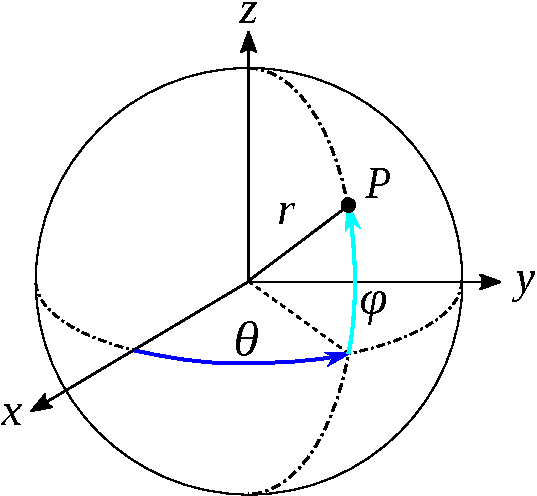
\includegraphics[width=0.35\linewidth]{../media/solidangle_cs.pdf}}
    \subfigure[Solid angle example graphic]{
        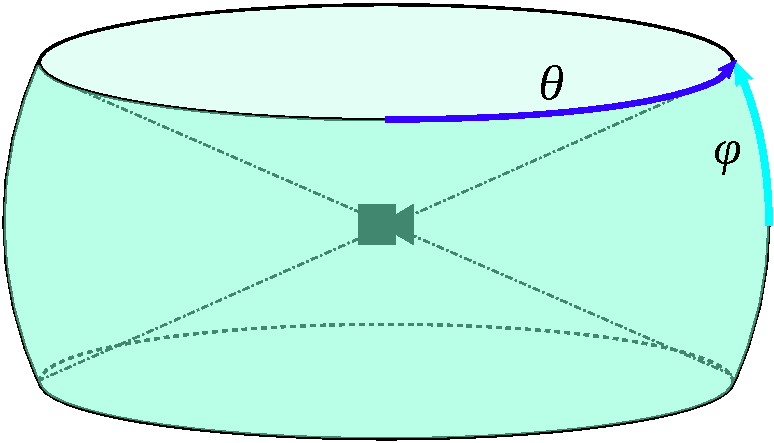
\includegraphics[width=0.5\linewidth]{../media/solidangle_ex.pdf}}
    \caption{(a) Spherical coordinate system for Equation \ref{eq_solidangle2}. (b) Example graphic demonstrating where angle values correspond to sensor. The transparent green region represents the sensor's visible field.}
    \label{solidangle}
\end{figure}

Given the information above, stereo sensors are the clear winner in terms of points per dollar (points/price) as well as point density (points/area).

On the question of quality, lidar becomes the de facto standard of measure due to its high accuracy.
This means that stereo vision quality is derived from how closely it matches a lidar scan. This also means that stereo vision quality is highly dependent on the system used, and can vary with both hardware and software implementation. A typical engineering threshold of 10\% is used for comparison, meaning that a single stereo-generated point is considered ``good" if its depth estimate is within $\pm$10\% of the absolute value of the corresponding lidar depth estimate. The horizontal and vertical distances, $x$ and $y$, are ignored due to the assumed 1:1 correspondence when projecting a point cloud onto the image plane. The steps to determine this quality are:

\begin{enumerate} \itemsep=-0.5em
    \item Project lidar points to image space, the resulting matrix named $L$
	\item Convert disparity values of stereo map to depth values, named $S$
	\item Keep only points from stereo map that also exist in $L$
	\item Aggregate depth pairs for as many images to compare as desired
	\item For each ($i=row,j=column$) index, calculate relative error with reference to lidar as given in Equation \ref{eq_errCalc}.
	\item Bin all results in 10 meter increments, relative to lidar values. In each subgroup, get the fraction of points within the bounds relative to the total number of points in the subgroup
\end{enumerate}

\begin{equation}
    e = \left | \frac{S_{i,j} - L_{i,j}}{L_{i,j}} \right |
    \label{eq_errCalc}
\end{equation}

After performing the following steps, Figure \ref{corr_pct_within} was generated: A bar graph of binned ranges and the fraction of stereo points in each range that within error tolerance of the reference lidar value.

\begin{figure}[ht]
	\centering
	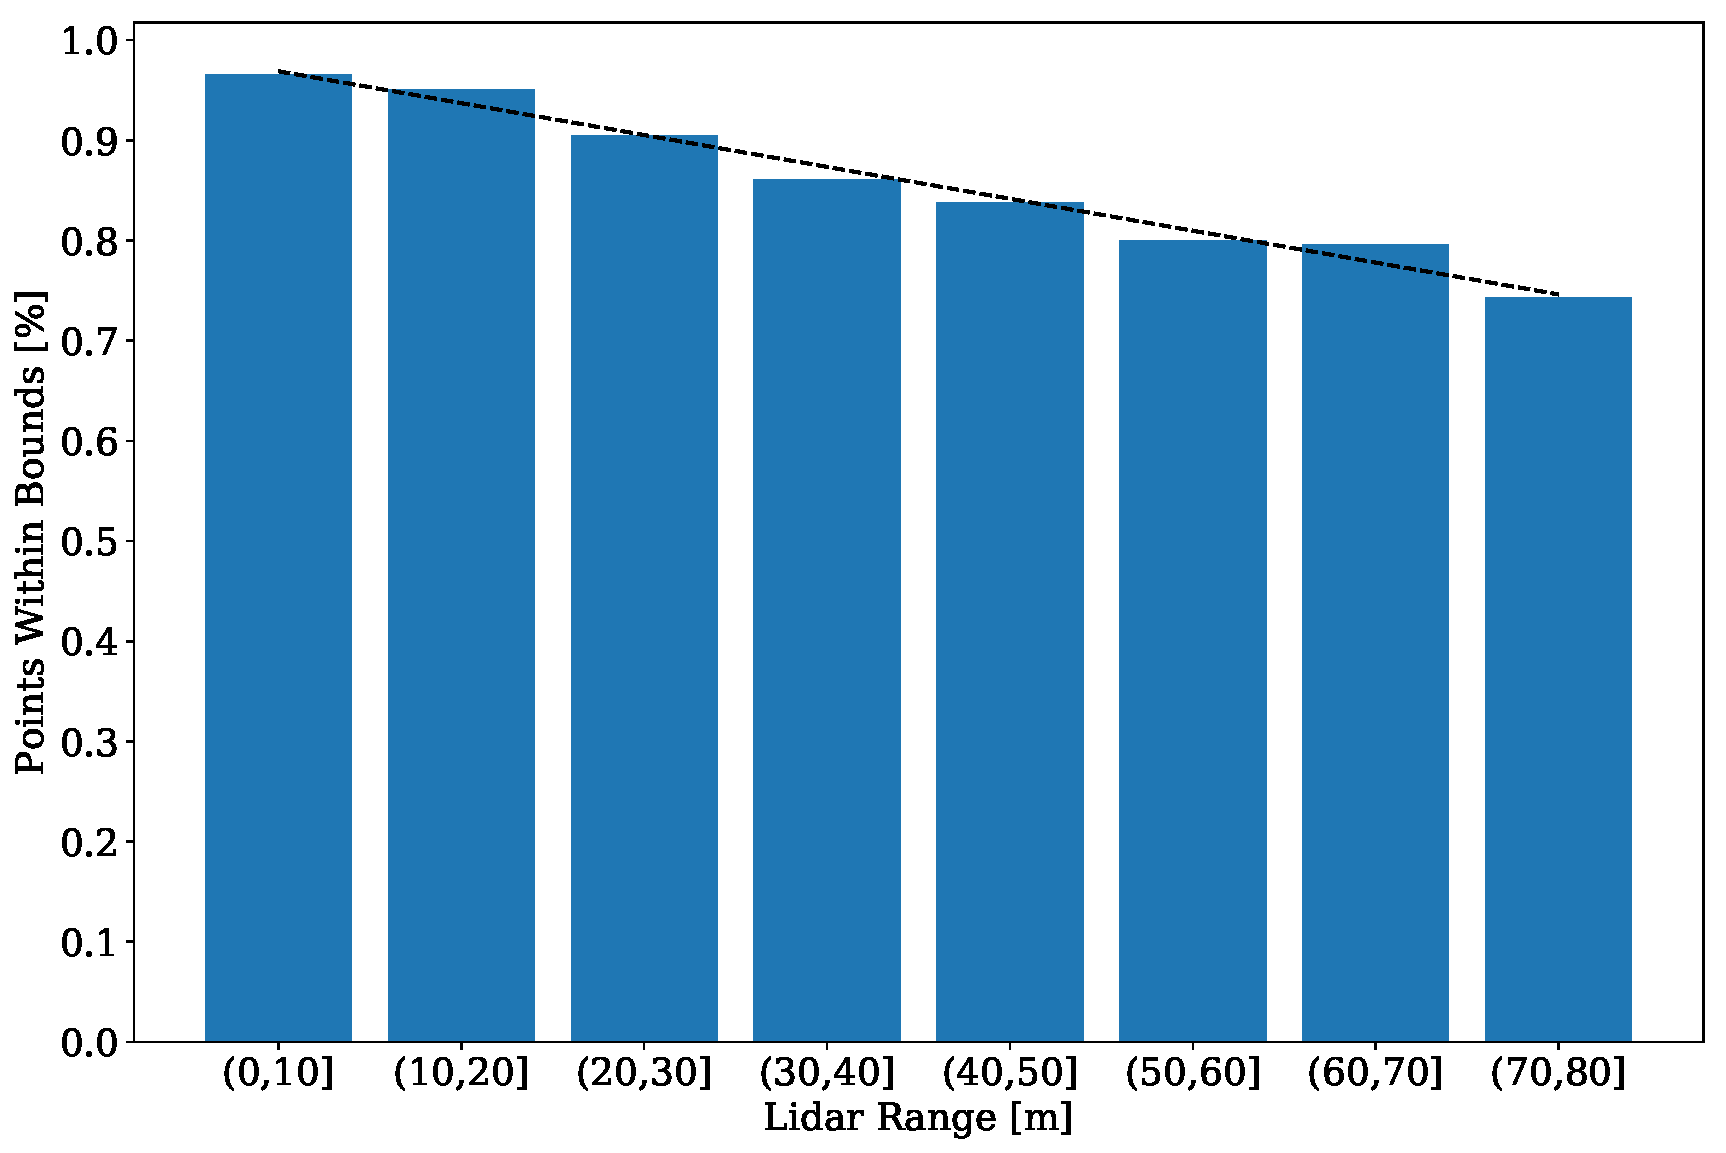
\includegraphics[width=0.8\linewidth]{../media/corr_pct_within.pdf}
	\caption{A bar chart describing what percentage of points lie within the given depth range. As an example, about 95\% of stereo depth values greater than 10 meters but less than or equal to 20 meters are within $\pm$10\% of the corresponding lidar depth value. The first 1000 indices of the KITTI dataset were used, altogether comprising 17,134,011 point comparisons between stereo and lidar. The dashed line indicates a 1st order polynomial fit, with the slope equal to about -0.03 percentage points per range (i.e. every 10 meters, there's about -0.03 change in percentage of points within bounds). In the smallest subset of points, the (70,80] range, there are 75,224 points. The fully developed Pyramid Stereo Matching network for use in Experiment 3 was used to generate part of the data.}
	\label{corr_pct_within}
\end{figure}

In summary, stereo vision is an attractive alternative to lidar vision because of its much higher point density, lower price, reasonable quality approximation of lidar, and the potential to improve through further research. Under the correct conditions, stereo vision sensors have the potential to compete with lidar sensors in terms of both quantity and quality.



% NEWSECTION ===================================================================
\newpage
\subsection{Related Work} % status: stereo vision, 3D, etc

\subsubsection{Stereo Vision}
Stereo disparity maps are built by comparing the pixel distance between two similar regions of two images. Generating a disparity map, however, was developed before the popularization of neural networks. The key step that most neural networks have been used to improve is matching cost computation \cite{chang_pyramid_2018},  one of the four typical steps as described by Scharstein \cite{scharstein_taxonomy_2002}. Out of this paper, the four main parts of conducting stereo vision have been classically defined as follows: matching cost computation, cost (support) aggregation, disparity computation and optimization, and disparity refinement.

Initially, built-in and readily available stereo disparity map computation techniques were used. In the Python OpenCV library, there is a ``Semi-global Block Matching" (SGBM) algorithm, implemented based on the paper by Hirschmuller \cite{hirschmuller_stereo_2007}. For an initial ``rough" pass, this algorithm was cheap and fairly effective. Additionally, this algorithm is useful for fast, fairly-stable calculations and does not need a GPU to run. However, it suffers from a few key shortcomings. For one, there is a large rectangular portion of the disparity map that contains no values, as can bee seen in the left side of Figure \ref{ind15_SGBM_comparison}(a), where missing values are marked red. Next, when a set of pixels cannot be matched between images, the result is simply a value of zero, giving no information in that region; these locations are also marked in red. Finally, SGBM suffers from a significant lack of resolution, meaning that some objects of interest, such as the three pedestrians in the image (highlighted with red rectangles in the color image), will not be seen well, or at all. For comparison, stereo images created with a neural network (NN) such as those in Figure \ref{new_psmnet} have a richer amount of information and have no missing pixels (i.e. a prediction is made at every pixel).

\begin{figure}[H]
    \centering
    \subfigure[SGBM disparity map]{
        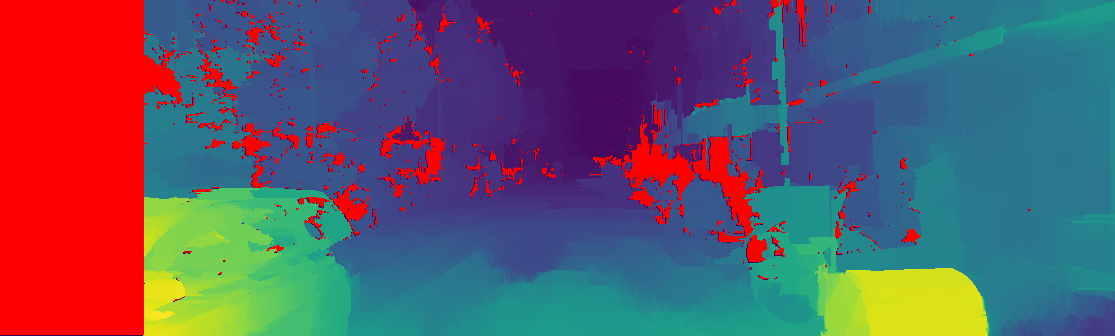
\includegraphics[width=1\linewidth]{../media/ind15_SGBM_comparison2.png}}
    \subfigure[LHS image]{
        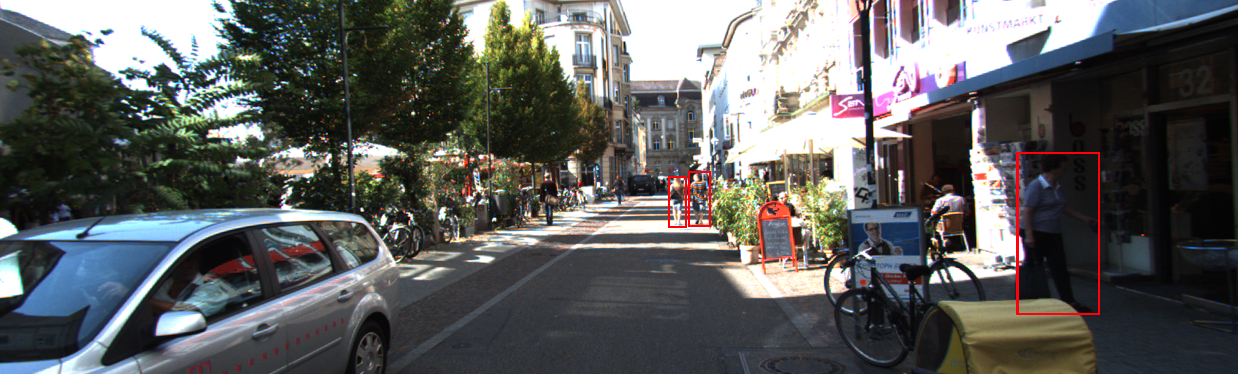
\includegraphics[width=1\linewidth]{../media/objdet_LHS_000015_withBox.png}}
    \caption{An example of a disparity map generated without a neural network approach. Though it has good merit, there are some noticeable shortcomings, with missing values colored red, uneven steps in value (car on left), and low resolution (three highlighted pedestrians not visible in map). This disparity map was generated in part by the left-side color image. Index 15 of the KITTI Object Detection dataset.}
    \label{ind15_SGBM_comparison}
\end{figure}

With this knowledge, the next step was to find an ideal NN-based stereo disparity estimation method. Notable stereo neural network approaches to disparity estimation include Pyramid Stereo Matching network (PSMnet) \cite{chang_pyramid_2018},  iResNet \cite{liang_learning_2018}, among others on the various stereo benchmarks. In order to select the best candidate, multiple benchmarks were considered. The first benchmark was naturally the KITTI Stereo challenge, which contains a list of the top performing networks. At the start of this thesis writing, PSMnet stood in the top 10 of stereo networks in this list \cite{menze_kitti_2019}.

\subsubsection{3D estimation with Stereo Disparity Maps}
There is currently a low amount of public research on stereo vision for use with 3D localization. Most approaches are typically derived from a lidar-based approach. Zeng, Hu, Liu, Ye, Han, Li, and Sun \cite{zeng2018rt3d} produced a stereo alternative to their original ``Real-Time 3D Vehicle Detection" network, yet had a difficult time adjusting the performance to account for the noise present in a stereo-generated point cloud, as their approach first transformed points into a bird's eye view (BEV), then performed detections. This approach essentially works on a 2D image of the desired area, using well-established 2D localization methods, but from a top-down view. Also working in 2D, but with a more traditional approach, Li, Chen, and Shen \cite{li_stereo_2019} takes the left and right images from each scene and obtains region proposals for both sides, eventually taking each proposal pair and estimating semantic information like ``object class, stereo bounding boxes, dimension", and so on. This approach does have its benefits, being deeply rooted in more traditional 2D localization techniques, such as those provided by Ren, He, Girshick and Sun \cite{ren_faster_2015}, but still experiences shortcomings due to working with three-dimensional data in a two-dimensional space. Additionally, some prior information is required, named as being a ``pre-set dimension prior" that is used for ``dimension prediction". In contrast, this thesis and the state of the art approaches avoid the need to have prior information about the world. Overall, the network seemingly has some difficulty learning to estimate information in at least one of the dimensions. In contrast to these previous approaches, the state of the art is currently achieved by Wang et al. \cite{wang_pseudo-lidar_2019} in an approach that reconstructs a stereo image into a point cloud, then manipulating the data in a three-dimensional space. Since the start of this paper, Wang et al.'s work became public knowledge, and was then published before this paper was completed. In the paper, ``Pseudo-LiDAR from Visual Depth Estimation", the authors took an extremely similar approach to this paper. Their network architecture takes a stereo image pair, generates a disparity map via Pyramid Stereo Matching network, converts it to a ``pseudo-lidar" scan, and extracts 3D bounding box estimations via Frustum Pointnet. This development unfortunately has a strong overlap with the contents of this paper, yet did not have origins in short-range detection of objects. However, in their paper, the authors argue that within a short distance, up to 30 meters away, stereo vision performs competitively with lidar, which is encouraging for the work performed here.

\subsubsection{3D Estimation with Lidar}
Performing 3D estimation and localization with lidar has been a focus for a large portion of the field, and with good reason. Lidar data, while expensive to obtain, currently provides the best option for 3D information. Thus, there are many papers which focus on using lidar sensor capabilities to estimate 3D bounding boxes, to varying degrees of success. As mentioned previously, Zeng et al. \cite{zeng2018rt3d} attempted to use lidar information with a novel 2D BEV approach, yet fell short of really taking advantage of the new dimension that lidar provided. The greatest breakthroughs have indeed been by networks that manipulate the information directly in the 3D space. Notably, Volumetric CNN's such as by Wu, Song, Khosla, et al. \cite{wu20153d} were one of the first leaps from 2D space to 3D space, using voxels created by the 3D information provided. However, this approach ultimately struggles with data sparsity and the massive computational cost of 3D convolution. Similar to the first two approaches named, multi-view CNN's such as by Su, Maji, Kalogerakis, and Learned-Miller \cite{su2015multi} attempt to use multiple 2D projections of the 3D space to estimate object locations. These also fail, namely when attempting to perform finer operations such as shape classification. One of the major successes in 3D object detection has been by Qi, Su, Mo, and Guibas \cite{qi_pointnet:_2017} in the development of Pointnets, a network that could directly and scalably ``summarize an input point cloud by a sparse set of key points". This had a built-in level of robustness, because the network was designed to operate on an orderless set of points, with less-than-complete knowledge of the 3D shape. However, an improvement came by the same authors when ``Frustum Pointnet" \cite{qi_frustum_2017} was introduced. This network simplified the classification process by first using a 2D object detector as a filter to isolate a region of the point cloud. This cone, or ``frustum", then allowed the Pointnet network to operate on a substantially smaller set of points, reducing computation time. This paper takes advantage of this capability to great effect, as explained in Section \ref{sect_fpnet}.

% NEWSECTION ===================================================================
\newpage
\section{Pyramid Stereo Network and Disparity Map Reconstruction} % topic1
\label{sect_psmnet}
The network developed over the course of this thesis, called Stereo Point Cloud Network (SPCLnet) can be broken up into two main sub-networks, as shown below in Figure \ref{spcl_arch}. The first sub-network is explained here, and the second sub-network is explained in the next section.

\begin{figure}[ht]
	\centering
	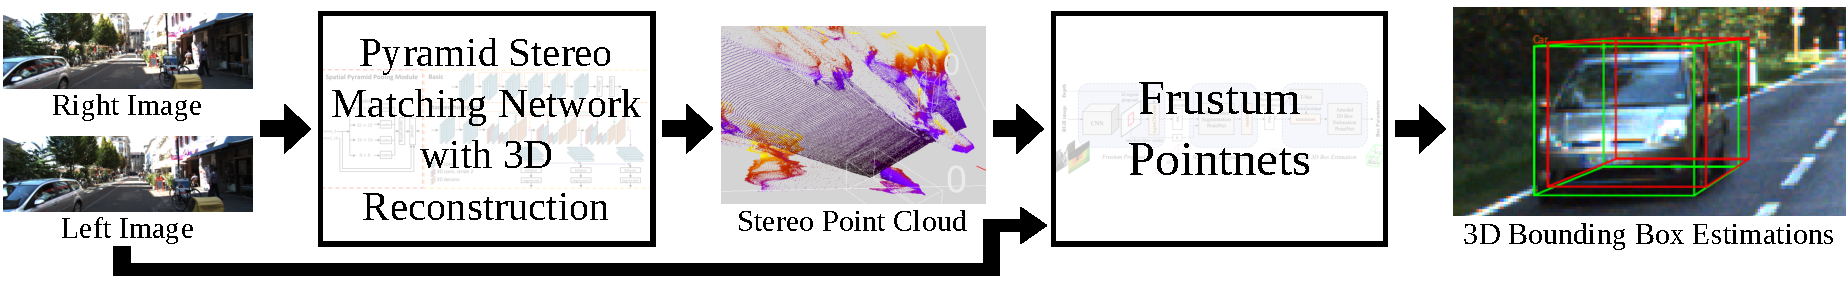
\includegraphics[width=1\linewidth]{../media/spcl_arch.pdf}
	\caption{General architecture of Stereo-Pointcloud network. A stereo image pair is fed to a disparity estimation network, specifically PSMnet, which then also reconstructs the disparity map into a 3D point cloud. The point cloud is then fed into a pointnet (along with the original left image), specifically Frustum Pointnet, which finally returns a 3D bounding box estimation. Images reproduced from \cite{geiger_are_2012}, \cite{chang_pyramid_2018}, and \cite{qi_frustum_2017}.}
	\label{spcl_arch}
\end{figure}

The first sub-network is used to generate a stereo-based point cloud from a disparity map estimation network, created by Chang and Chen \cite{chang_pyramid_2018}. The majority of the following information is derived from their work. This sub-network consists primarily of a ``Spatial Pyramid Pooling module" to look for matching information at various levels of detail, as well as a ``stacked hourglass module for cost volume regularization". After the sub-network is described, a brief explanation of reconstruction is also provided. 

\subsection{Pyramid Stereo Matching Network Architecture}
The first task in creating a network that can take a stereo image pair and generate 3D bounding boxes, as described in Figure \ref{spcl_arch} above, is to have the capability of taking a stereo image pair and creating a disparity map. To that end, a best-in-class disparity generation algorithm was searched for and selected to be the Pyramid Stereo Matching Network (PSMnet). This network takes a deep learning approach to generating disparity maps from a pair of images. The network itself is near the top of the state of the art, and achieves this by the architecture of its network. The openly-available repository provided a foundation to start on towards making a compact, easy-to-use function.

First, the original evaluation code was tested out. Some modification and housekeeping had to be done to ensure that it was compatible with the local installation, as well as being adapted for use with Python 3. All deprecated functionality was manually removed. Finally, a self-made set of ground-truths were eventually generated in order to train the network on the KITTI Object Detection dataset instead of the Stereo dataset. This was done by projecting lidar points onto the image plane, removing points outside image bounds, and multiplying appropriate factors as outlined in the development kit. This is also clarified in Section \ref{sect_datamod}.

Pyramid Stereo Matching Network, or PSMnet, is a network that takes advantage of an hourglass-shaped network. The result are very high quality, high resolution disparity maps. The network takes advantage of GPU processing power, depending on NVIDIA's GPU acceleration, similar to other networks. The network itself is written in PyTorch, a flexible and python-based network module which enabled simplified debugging. PSMnet's architecture is shown below in Figure \ref{psmnet_arch}.


\begin{figure}[ht]
	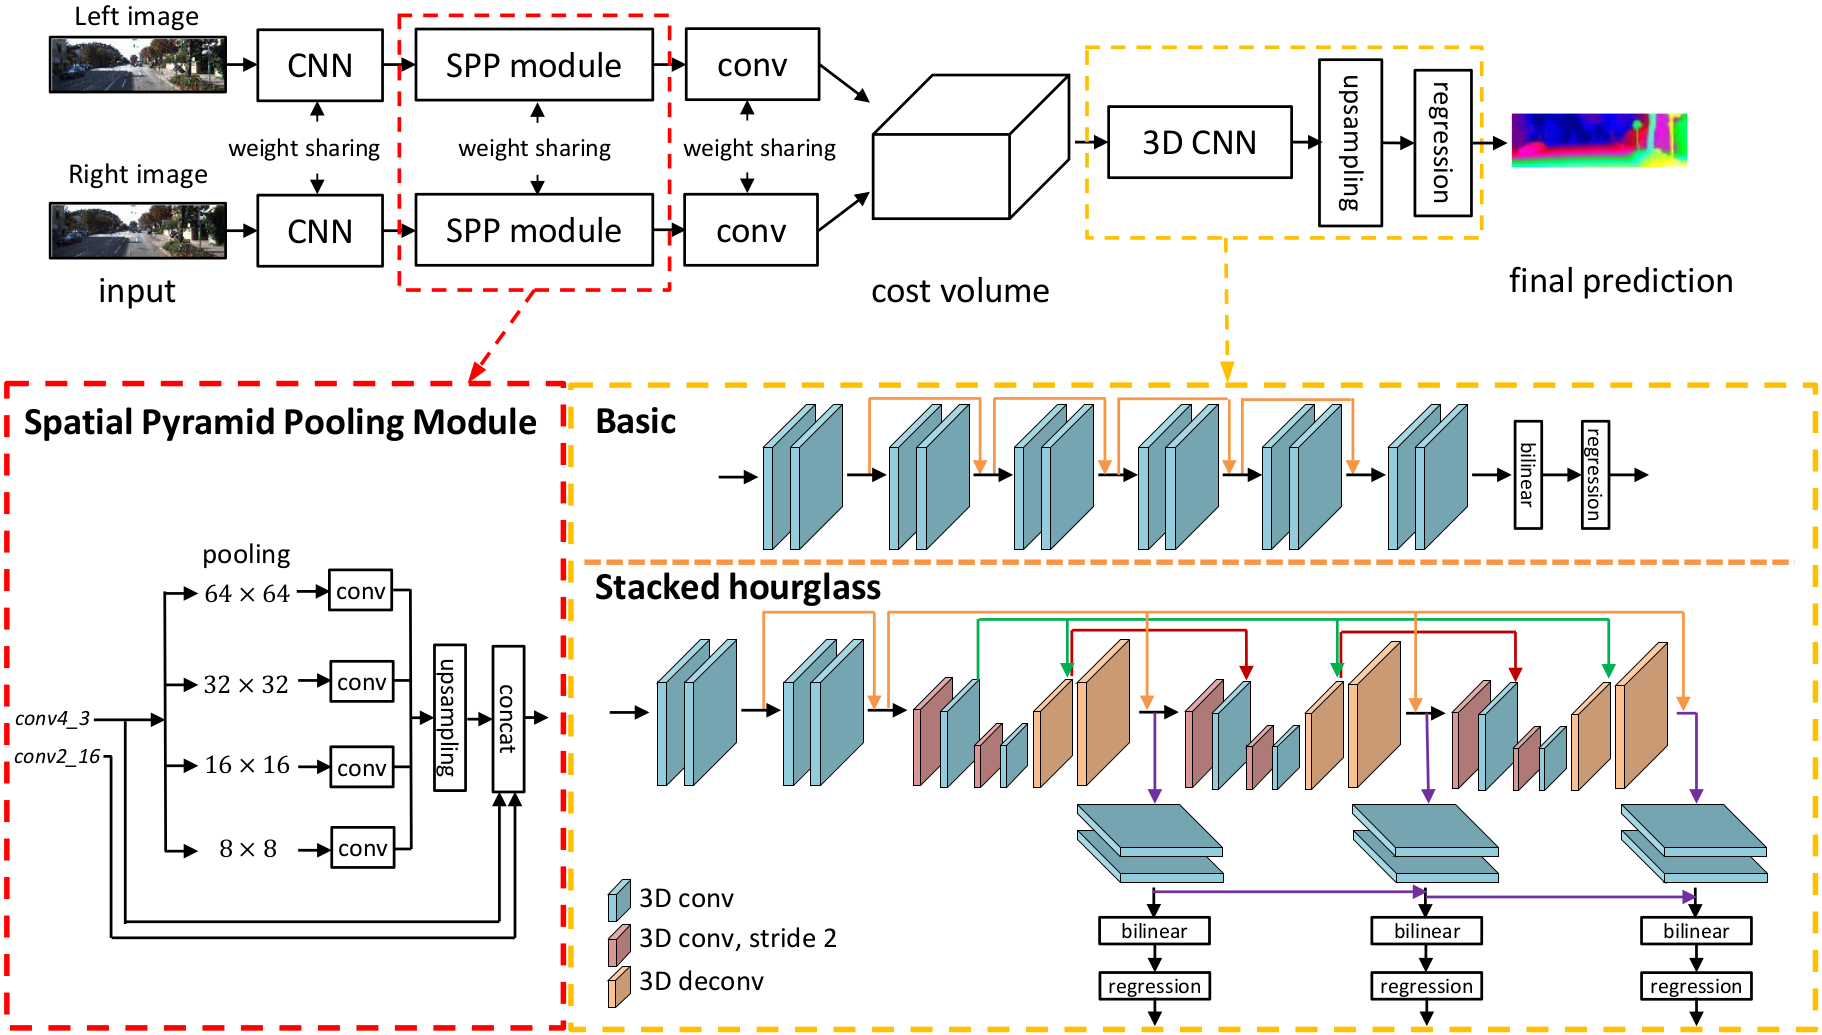
\includegraphics[width=1\textwidth]{../media/psmnet_arch.png}
	\caption{Generalized network architecture for Pyramid Stereo Matching network. The 3D CNN has two available configurations, Basic and Stacked hourglass. Stacked hourglass was used here. The Spatial Pyramid Pooling Module helps describe how features at varying magnification levels were concatenated together. Image reproduced from \cite{chang_pyramid_2018}.}
	\label{psmnet_arch}
\end{figure}


To properly understand PSMnet, the network will be explained in three general steps, as described by the original authors Jia-Ren Chang and Yong-Scheng Chen \cite{chang_pyramid_2018}. 

\begin{enumerate}\itemsep=-0.5em
    \item Initial 2D convolution into Spatial Pyramid Pooling 
    \item Aggregate all data into a cost volume
    \item Perform 3D convolution and ``deconvolution" on the cost volume until a final prediction is reached.
\end{enumerate}

\textbf{{\large Step 1: Spatial Pyramid Pooling (SPP) Module}} \\
To begin finding a disparity map from an image pair, the images each fed into a 2D CNN with weight sharing (meaning that the two CNN's have identical weights). The two images are thus changed from
color images with dimensions (Height, Weight, Channel=3) to feature maps with dimensions (H/4, W/4, Features=32). These two maps which are then each fed into a SPP module, which uses average pooling to capture details of each map at various scales. In effect, the SPP module ``zooms" at various magnifications in order to capture different levels of detail in the same image, all of which are then concatenated together, along with the original feature map, into an aggregated feature map. At this point, there feature dimension is rather large, expanded to 320 from 32. Additional convolution with a 1x1 filter size helps reduce the number of features back down to 32, and each aggregated feature map is sent into the cost volume to be further combined.

The primary reason for the SPP module is to take advantage of ``image features rich with object context information" \cite{chang_pyramid_2018} while addressing the fixed-size constraint of CNN's. By looking at the image at various magnifications, the network learns to ``incorporate hierarchical context information", such as an object like a car and its sub-objects like tires, windows, and so on. At this point, the network is not yet calculating anything like disparities, but rather learning the relationships between sub-regions that may later play a part in determining distance relationships between them.

\textbf{{\large Step 2: Cost Volume}} \\
Next, the two aggregate feature maps are combined into a single 4-dimensional matrix known as a cost volume. As described by Chang and Chen, the left and right feature maps are concatenated, resulting in a 4D ``volume", with dimensions (Height, Width, Disparity, Features). The disparity level is created from the various scales at which features are concatenated, or ``levels" as the paper describes. Later on, these disparity values will be refined into a final estimate via regression. The usage of a cost volume will later necessitate the use of a 3D convolution, to deal with the extra dimension generated. At this point, the cost volume has a general shape of (D/4, H/4, W/4, 64), as described by Table 1 in the original paper \cite{chang_pyramid_2018}.

\textbf{{\large Step 3: 3D Convolutional Neural Network}} \\
The last major step of PSMnet is to take the cost volume and perform stereo matching. At this point, the task has been somewhat simplified by using an SPP module at the start in order to involve ``different levels of features" \cite{chang_pyramid_2018}. There are two 3D CNN architectures that the authors developed, a ``Basic" and ``Stacked Hourglass" architecture. This thesis used the ``Stacked Hourglass" network for its improved performance. In brief summary, the Basic 3D CNN is comprised solely of residual blocks that convolve the cost volume. This reduced cost volume is then upsampled up to a shape of (Height, Width, Disparity), and finally regression is used to ``calculate the disparity map with size H x W".

The Stacked Hourglass architecture, in contrast to the Basic architecture, uses two kinds of convolutional layers along with complimentary transposed convolutional layers to repeatedly reduce and upsample the cost volume. Figure \ref{psmnet_hourglass} below reproduces just the Stacked Hourglass network from Figure \ref{psmnet_arch} above. 


\begin{figure}[ht]
	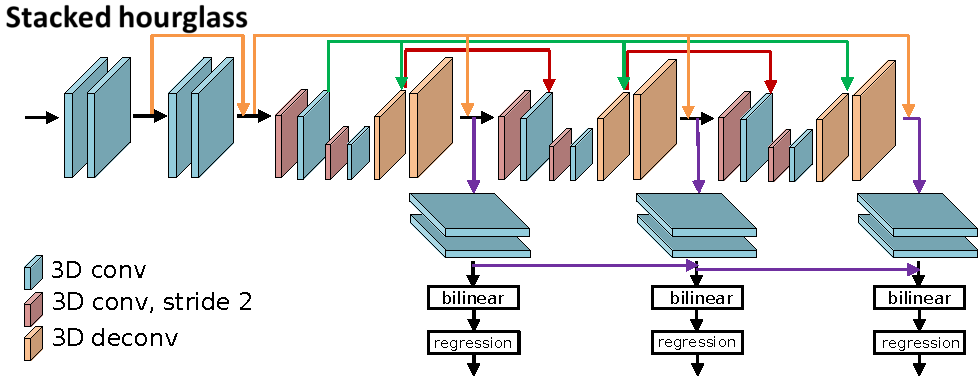
\includegraphics[width=1\textwidth]{../media/psmnet_hourglass.pdf}
	\caption{Detailed view of Stacked Hourglass architecture from PSMnet. Image reproduced from the PSMnet paper \cite{chang_pyramid_2018}.}
	\label{psmnet_hourglass}
\end{figure}

The first four layers (marked in blue) are 3D convolutional layers with a stride of 1. The disparity, height, and width dimensions don't change, but the number of features are reduced from 64 to 32. Next, the network actually begins its ``hourglass" portion, with a 3D convolutional layer of stride 2 (marked red) halving the Disparity, Height, and Width dimensions (by half) while doubling the Features. This step is again repeated (without changing the Features size), bringing the dimensions to (H/16, W/16, D/16, Features=64). 

This is the ``smallest" that the cost volume will be, and it is next upsampled via 3D transposed convolution, or 3D ``deconvolution" as it is also known. The simple reason that this network is upsampled using deconvolution is to reconstruction predictions about the disparity at a higher resolution. This is similar to how a low-resolution image may be upsampled into a higher resolution, requiring some kind of calculation to estimate the true value of unknown pixels. In the same way, deconvolution expands the cost volume again to correct the shrinking that happens with convolution. However, in order to recover some information about the values lost from the hi-res cost volume, a ``skip layer" is also implemented. Skip layers, in a practical sense, are an operation to take the weights from a previous layer and add them element-wise to a future layer later on. This is best exemplified by the green arrows in Figure \ref{psmnet_hourglass}, although the orange and red arrows are also skip layers. Thus, features that may have been lost during convolution are partially restored during deconvolution. 

Once the cost volume has been reduced and then upsampled in size, a single hourglass step has been taken. This hourglass shape is also known as an encoder-decoder architecture, popularized by SegNet, an architecture for image segmentation by Badrinarayanan, Kendall, and Cipolla  \cite{badrinarayanan_segnet:_2017}. In their paper, the authors argue that the key component is ``the decoder network which consists of a hierarchy of decoders one corresponding to each encoder", enabling the ability to perform non-linear upsampling while still being memory efficient. The ``stacked" nature of PSMnet comes from repeating this hourglass network multiple times, three in total. 

Each time the network is upsampled, it outputs a new cost volume. Each of these cost volumes, eventually becoming disparity maps, are optimized during training. In testing, the final cost volume is used. This cost volume is then upsampled in a bilinear fashion, and finally the continuous disparity map is calculated via ``disparity regression". The authors of PSMnet utilize this as described by Kendall et al. \cite{kendall_end--end_2017}: in contrast to estimating disparity with an argmin operation, Kendall defined a differentiable ``soft argmin" function and capable of creating sub-pixel disparity estimates. Although the details of this operation will not be explained here, Chang implements this in PSMnet to collapse the four-dimensional cost volume into a two-dimensional disparity map. 

\subsection{3D Reconstruction from Stereo Data}
\label{sect_reconstruct}
%things to cover: 
%1. introduction to reconstruction and methods
%2. where explained and referenced
%3. start with simple image describing the initial problem
%4. give equations, with explanation of variables
%5. give more concrete example of how one performs this, with both a disparity image and a given point cloud.
Reconstruction is the process of taking a series of 2D images and producing a 3D representation of that information, as explained by Szeliski \cite{szeliski_computer_2010}. Here, the main goal is to end up with a point cloud, an unordered set of metric coordinates. Epipolar equations, equations derived from the geometrical relationship two cameras viewing a single scene, allow one to perform these conversions, which are explained below.

The overall steps of reconstructing the resulting stereo image consists of three general equations adapted for use with matrix operations\cite{szeliski_computer_2010, wang_pseudo-lidar_2019}. This also includes selecting the proper constants for each calculation. To achieve all this, a specific Python class was created that would initialize by loading the fully trained model and use it in a non-learning ``testing" mode, whereby it would take in either an image path pair or a loaded pair of image arrays. The pair would then be evaluated in PSMnet, and the resulting disparity map would be converted to a point cloud using the epipolar equations in matrix form. Each record of the KITTI dataset has its own calibration file, but the baseline value remains the same.

To begin describing how the transformation is done, a simple problem is presented with the following assumptions. Let there be two cameras in a scene, both facing the same direction and able to see an object at point $P$, such as a ball. The following assumptions are made: 

\begin{itemize} \itemsep=-0.5em
	\item The two cameras are identical in performance, producing equal quality images at the same point in time.
	\item The camera centers are aligned (for simplified rectification).
	\item Images produced are already rectified (to remove all distortion). Rectification involves using the camera's intrinsic properties in order to correct lens distortion, specifically barrel distortion.
	\item The camera centers $O_i$ are separated by a baseline distance $b$.
	\item The two cameras have identical horizontal focal lengths $f_U$.
	\item The ball appears at some horizontal distance $u_i$, whether the origin is measured from the left side of the image or the center.
\end{itemize}

When the two cameras take an image of the ball, the light rays they capture may be drawn as given in Figure \ref{epipolar}. The figure gives a top-down view of what both cameras capture, and the horizontal pixel location at which the light ray comes into contact with each camera center. 

\begin{figure}[ht]
    \centering
	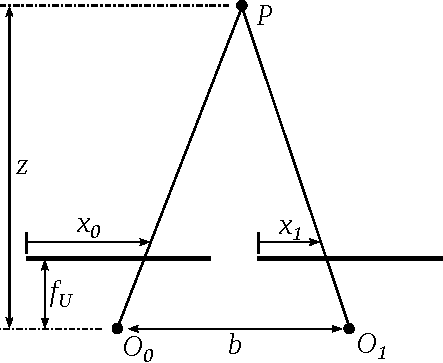
\includegraphics[width=0.4\textwidth]{../media/epipolar.pdf}
	\caption{Simplified graphic demonstrating how disparity may be derived from two cameras. The images the cameras produce must first be rectified.}
	\label{epipolar}
\end{figure}

Given the above physical setup, the equation describing the relationship between disparity and depth $z$ may be found. When a matrix of disparity points is given, denoted as $D$, the resulting equation is then: 
\begin{equation}
z = \frac{f_U b}{D}
\label{eq_epi_z}
\end{equation}

Thus, a depth map may be generated by using this equation on each disparity value. The process of determining horizontal distance $x$ and vertical distance $y$ requires further exploitation of the camera geometry, and may be calculated then as: 
\begin{equation}
x = \frac{z (u - c_U)}{f_U}
\end{equation}

\begin{equation}
y = \frac{z(v - c_V)}{f_V}
\end{equation}

It is important to note that $f_U$ and $f_V$ are for horizontal and vertical focal lengths (respectively), ($c_U$,$c_V$) are the pixel center of the image, and $(u,v)$ represent a (column, row) coordinate location in $D$ with the origin at the image's top-left corner.

In practice, the calculation is performed in a series of matrix calculations rather than as an element-by-element operation. These steps are covered below with accompanying Python code. This code assumes the usage of the Numpy module and that the disparity map has already been generated and saved.

The first step in the reconstruction process is determining the baseline, focal lengths, and image center. The baseline is a given constant from the KITTI development kit, listed as a fixed value of 0.54 meters. The accuracy of this measurement is not known beyond that. For each scene, the focal lengths are determined directly from the left color camera calibration matrix $P_2$, where $f_U=P_2[0,0]$ (row 0, col 0) and $f_V=P_2[1,1]$. The image centers are found by dividing the disparity dimensions by half of the image dimensions, which corrects for non-standardized image dimensions present throughout the dataset. The depth matrix $Z$ is calculated via matrix operations in nearly the same way as given in Equation \ref{eq_epi_z}. All code used below and throughout this work can be found in the thesis Gitlab repository \cite{gonzalez_smart3d_2019}. 
\begin{lstlisting}
import numpy as np
# STEP 1: generate / load a disparity map
disp=np.load(dpath)

# STEP 2: obtain parameters
P2 = rec.P2 # pre-existing object that parses calibration file
fHoriz = P2[0,0]
fVert= P2[1,1]
Baseline = 0.54 # meters. Obtained from devkit
imH,imW = np.array(pil.open(lpath).convert('RGB')).shape
Cu=disp.shape[1]-imW/2 # Cu = imW/2 - (imW - dispW)
Cv=disp.shape[0]-imH/2 # Cv = imH/2 - (imH - dispH)

# STEP 3: Calculate depth from disparity values
zvals = fHoriz*baseline/disp
\end{lstlisting}

Next, the $X$ and $Y$ matrices are generated by creating a vectorized forms of their corresponding theoretical equations: 
\begin{lstlisting}
# STEP 4: Convert x_px & y_px to metric
xpos=np.arange(0,zvals.shape[1])-Cu
ypos=np.arange(0,zvals.shape[0])-Cv
ulocs=np.tile(xpos*-1,(zvals.shape[0],1))
vlocs=np.tile(ypos*-1,(zvals.shape[1],1)).T
xvals = ulocs*zvals/fHoriz
yvals = vlocs*zvals/fVert
\end{lstlisting}

Once each matrix has been created, they may be combined to form a set of three dimensional coordinates, as shown below in Figure \ref{reconstruction}(e). 

\begin{figure}[H]
    \centering
    \subfigure[left image]{
        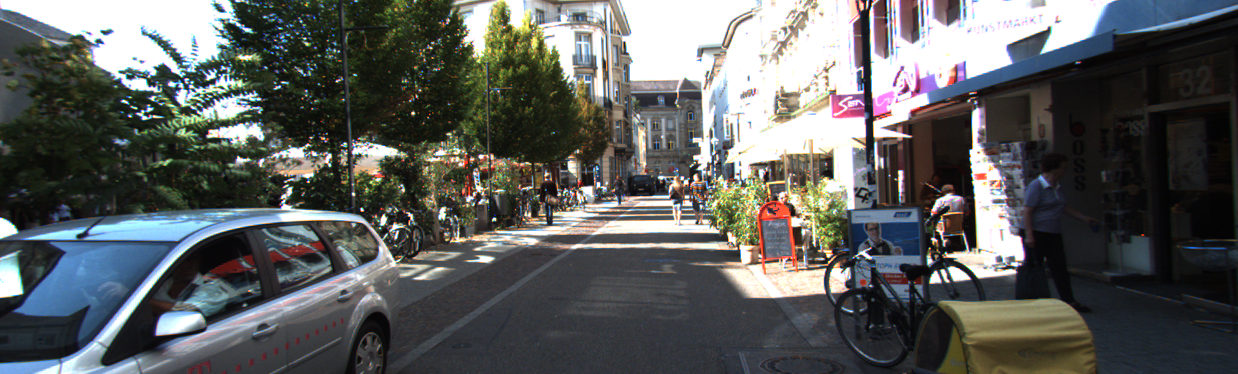
\includegraphics[width=0.487\linewidth]{../media/objdet_LHS_000015.png}}
    \subfigure[right image]{
        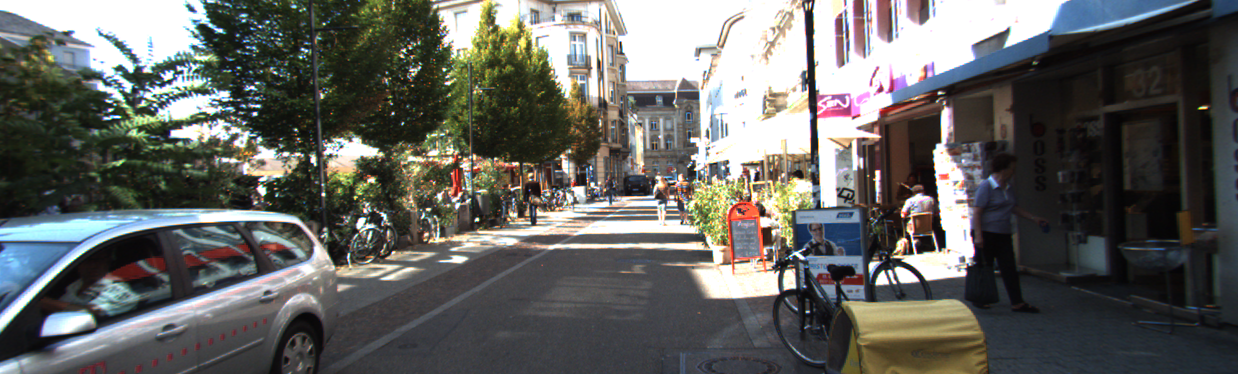
\includegraphics[width=0.487\linewidth]{../media/objdet_RHS_000015.png}}
    \subfigure[disparity map]{
        
\includegraphics[width=0.487\linewidth]{../media/ind15_psmstar_v190613_AsOf190626.png}}
    \subfigure[depth map]{
        
\includegraphics[width=0.487\linewidth]{../media/ind15_disp2depth.png}}
    \subfigure[final point cloud result]{
        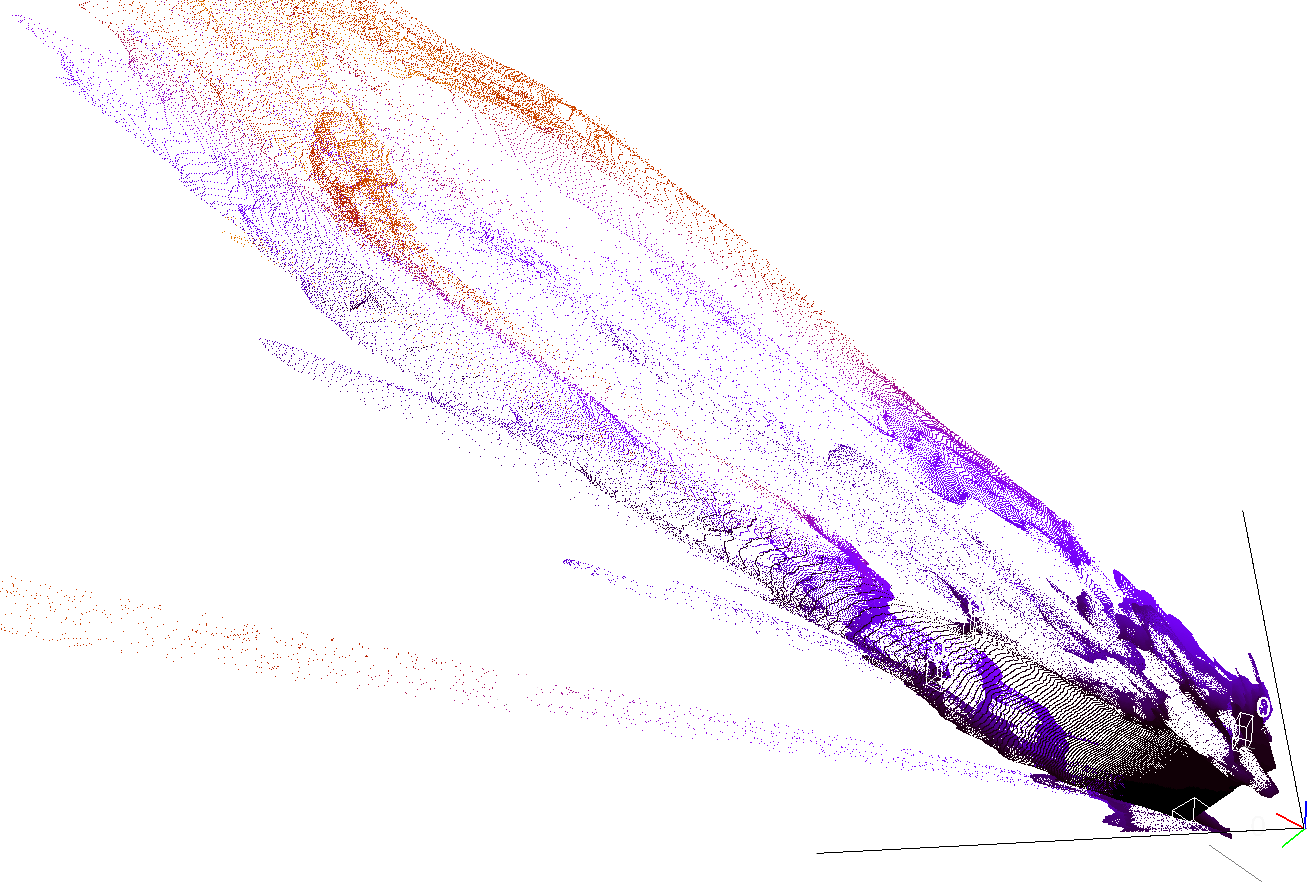
\includegraphics[width=1\linewidth]{../media/ind15_disp2pcl.png}}
    \caption{Various states of transformation from an image pair to a point cloud. Two images, (a) and (b) are given to PSMnet, which outputs a disparity map (c), which is changed to a depth map (d) via \ref{eq_epi_z}, and is finally transformed into a point cloud (e) with the remaining two epipolar equations. Subfigure (e) shows the camera horizontal field of view with two black lines.}
    \label{reconstruction}
\end{figure}






% NEWSECTION ===================================================================
\newpage
\section{Frustum Pointnet and Point Clouds} % topic2
\label{sect_fpnet}

Frustum Pointnet (FPnet) is one of the top-performing 3D object estimation networks on the KITTI Object Detection leaderboard. It's power comes from the ability to work with an incomplete or even reduced set of point data while still taking advantage of mature 2D object detection techniques. The network will be described in detail here, with the general architecture of FPnet is shown below in Figure \ref{fpnet_arch}, reproduced from the original paper by Qi et al \cite{qi_frustum_2017}. 

\begin{figure}[H]
    \centering
    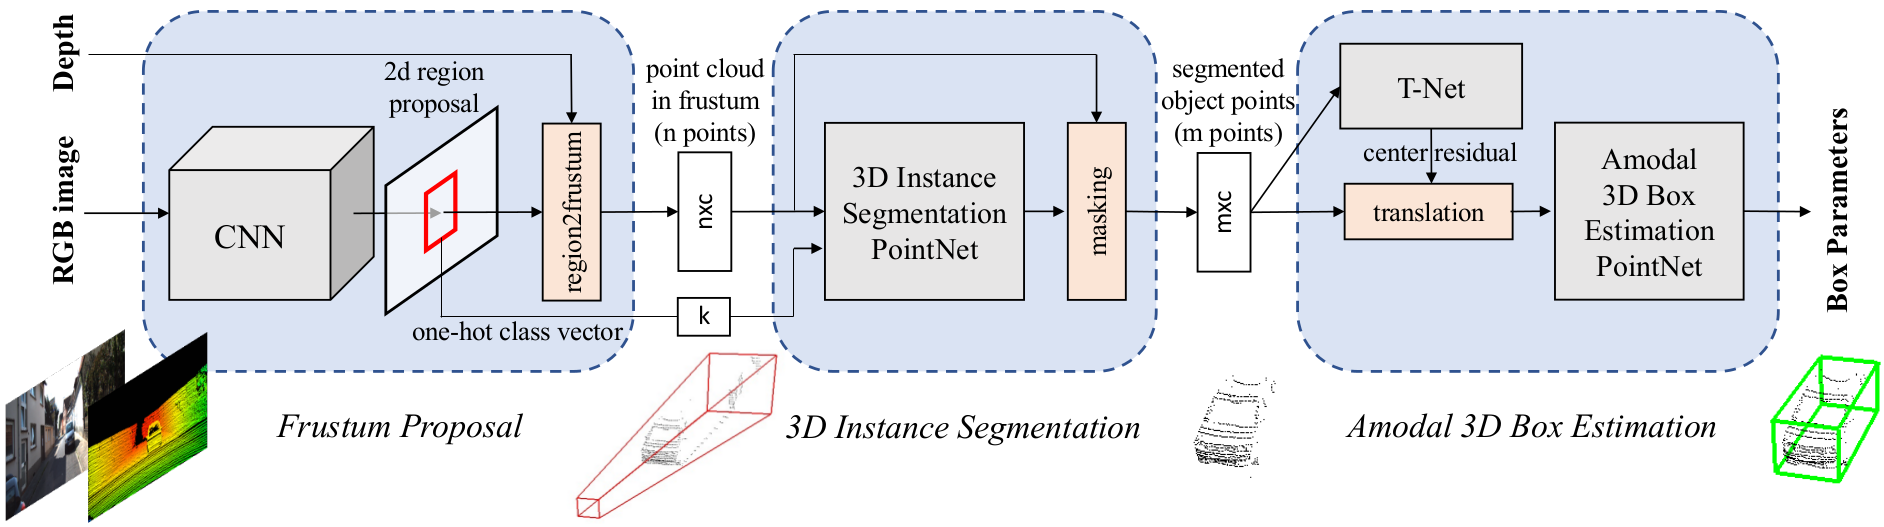
\includegraphics[width=1\textwidth]{../media/fpnet_arch.png}
    \caption{Frustum Pointnet architecture. Reproduced from original paper \cite{qi_frustum_2017}.}
    \label{fpnet_arch}
\end{figure}

\subsection{Frustum Pointnet Architecture}
The network itself works in three separate but closely related steps: 
\begin{enumerate}
    \item Frustum Proposal: A 2D CNN takes an RGB image and localizes a set of detections as region proposals, also generating a ``one-hot" class vector that determines which classes are searched for in the next step.
    \item 3D Instance Segmentation: For each region proposal, a cone or ``frustum" is cut out from the point cloud, a and a 3D instance segmentation is performed, and a masking step removes both needless foreground and background points.
    \item Amodal 3D Box Estimation: Each filtered subset of the point cloud is then subjected to amodal 3D box estimation, meaning that the incomplete set of points are then used to estimate a final set of 3D bounds defining the estimate for each detection.
\end{enumerate}

\textbf{{\large Step 1: Frustum Proposal}} \\
The very first step of FPnet requires a subnetwork, a 2D object detector, in order to begin generating proposals. The exact nature of this detector can be swapped for any 2D detector, such as R-CNN, SSD, etc. but the core step is to obtain 2D pixel-wise bounding boxes of target classes. Per the authors, an Feature Pyramid Network model is used to determine these bounding boxes, developed by Lin, Dollár, Girshick, He, Hariharan, and Belongie \cite{lin_feature_2017}. As described by Qi et al., they ``pre-train the model weights on ImageNet classification and COCO object detection datasets and further fine-tune it on a KITTI 2D object detection dataset to classify and predict amodal 2D boxes." \cite{qi_frustum_2017}.

Once these bounding boxes have been created, called ``2D region proposals", they are reconstructed into cone-like volumes called frustums via a custom-made function. In combination with the raw depth map, sub-cloud is created for each region proposal along with a ``one-hot class vector", essentially passing on the 2D information about each frustum. 

This step is straightforward enough, and the reasoning is obvious: 2D object detection has matured much faster than that of 3D, to the point that some 2D detectors can run in real-time with an average precision over 90\%. This reduces the search space from an entire lidar scan down to a narrow cone of points. As stated by Qi et al, ``the computational complexity of 3D search typically grows cubically with respect to the resolution and becomes too expensive for large scenes or real-time applications" \cite{qi_frustum_2017}.


\textbf{{\large Step 2: 3D Instance Segmentation}} \\
Once a set of sub-level point clouds and their respective class vectors have been generated, this sub-cloud must be further filtered by removing ``clutter". The core task here is to remove foreground and background points, which is implemented via a ``PointNet-based" network and whose sub-architecture is shown in Figure \ref{fpnet_subarch}(a). Pointnet, as developed by Qi, Su, Mo and Guibas \cite{qi_pointnet:_2017}, is capable of taking a point cloud and creating a ``probability score for each point that indicates how likely the point belongs to the object of interest" \cite{qi_frustum_2017}. Pointnet is itself a special type of spatial transformer network (STN), based on the work by Jaderberg, Simonyan, Zisserman, and Kavukcuoglu \cite{jaderberg_spatial_2015}. STN's are designed to transform data (scale, rotate, flip, etc), and learn how to do so as part of a larger network architecture. This enables some unique and powerful classification capability, where the network learns to first reshape the data before attempting to classify it. 

There is an added benefit to Pointnet as well: each sub-cloud has a prior category that is believed to be the primary subject of that sub-cloud, such as a car or pedestrian. The network can then learn to look for ``car-like" points, based on the prior training. Pointnet itself is a robust network model that can handle point corruption, extra noise points, and even reduced points when segmenting objects. As shown below in Figure \ref{fpnet_segmentation}, the network learns to remove occlusion (foreground noise) and clutter (background noise). The result from this step is a smaller sub-cloud of segmented object points along with all previous class information. 

\begin{figure}[H]
    \centering
    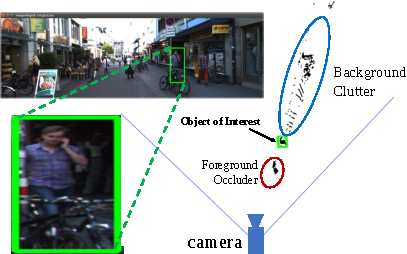
\includegraphics[width=0.5\textwidth]{../media/fpnet_segmentation.pdf}
    \caption{Frustum Pointnet 3D segmentation example. Reproduced from original paper \cite{qi_frustum_2017}.}
    \label{fpnet_segmentation}
\end{figure}

This is an important step in the detection pipeline because the network must be able to remove noise since the next step, amodal estimation, depends on having as little extraneous information as possible. This step is a 3D analog of the 2D segmentation task, where each pixel is either included or excluded as a part of the target class. Additionally, the origin of these points is transformed from the sensor coordinate to a local ``3D mask" coordinate (centered at the sub-cloud centroid and oriented in the same direction as the frustum), while also learning to recognize the general geometry of an object of a certain category \cite{qi_frustum_2017}.

\textbf{{\large Step 3: Amodal 3D Box Estimation}} \\
The final step in FPnet is to perform amodal 3D box estimation, meaning the estimation is done with incomplete or missing data. This step is performed in two parts: a ``light-weight" version of Pointnet named ``T-Net" is used solely to estimate the actual center of the object from the given sub-cloud, and then this transformed set of points is run through another Pointnet to estimate the final 3D bounds. Both the center-estimation step an the bounding box step are supervised separately. The T-Net and the amodal estimation Pointnet are shown below in Figure \ref{fpnet_subarch}(b) and (c), respectively. 

T-Net is a lightweight version of Pointnets, and has the sole task of estimating the ``true center" \cite{qi_frustum_2017} of the object, which is then set a the origin. Object priors are not used here; instead, supervised learning teaches the network to estimate the general size of the object, given only the sub-cloud set of points. This better prepares the next Pointnet to then predict the all parameters for bounding box estimation: object center ($c_x,c_y,c_z$), size ($h,w,l$) and heading angle $\theta$ \cite{qi_frustum_2017}. The bounding box center is later refined by combining the various residual centers from previous transforms. 

The need to change the residual center stems from empirical proof that the network learns how to estimate the object orientation much better when this step is enabled. The original paper demonstrates (in Table 8 of the source) that there is an accuracy improvement from 12.5\% to 74.3\% by including the various sub-nets to rotate and recenter the origin, strongly implying that the network needs to work with a local origin rather than a global one to better learn its parameters. 

 \begin{figure}[ht]
 	\centering
    \subfigure[]{
	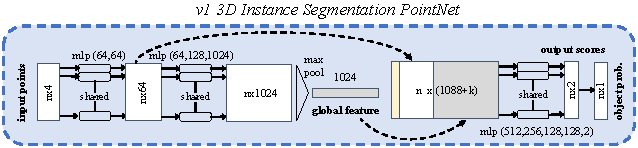
\includegraphics[width=0.95\linewidth]{../media/fpnet_subarch_segmentation.pdf}}
    \subfigure[]{
	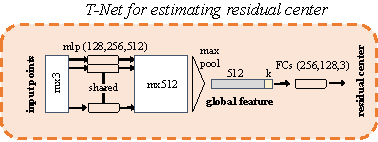
\includegraphics[width=0.487\linewidth]{../media/fpnet_subarch_tnet.pdf}}
    \subfigure[]{
	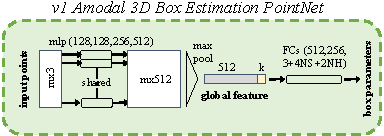
\includegraphics[width=0.487\linewidth]{../media/fpnet_subarch_estimation.pdf}}
 	\caption{Frustum Pointnet sub-networks. Reproduced from original paper \cite{qi_frustum_2017} Subfigure (a) is the architecture used during instance segmentation: removing foreground and background noise. Subfigure (b) shows T-Net, used for estimating the true object center. Subfigure (c) represents the final Pointnet, used to estimate the object's local bounding box values.}
 	\label{fpnet_subarch}
 \end{figure}

\subsection{Modification of Frustum Point Net}
Frustum Pointnet, being originally written for Python 2, needed to undergo some minor adaptations for usage with Python 3. Additionally, several modules and functions were deprecated or needed modification, and so had to be properly adapted. There are also two actively maintained versions of the Frustum Pointnet code. as explained in the original paper \cite{qi_frustum_2017}: the first which uses standard Tensorflow libraries and is based off Pointnets \cite{qi_pointnet:_2017}, and the second which uses custom Tensorflow operators that must be compiled, based off Pointnets++ \cite{qi_pointnet++:_2017}. For the purposes of this paper, version 1 was used.

In order to transition from using the provided pre-trained model and preprocessed data to self-made preprocessed and trained data, a set of steps and ``paths" were created to guide what was happening in each step and set of ``runs". As shown below in Figure \ref{fp_paths}, there are various steps with a gradual transition to stereo-based point cloud data.

\begin{figure}[H]
    \centering
    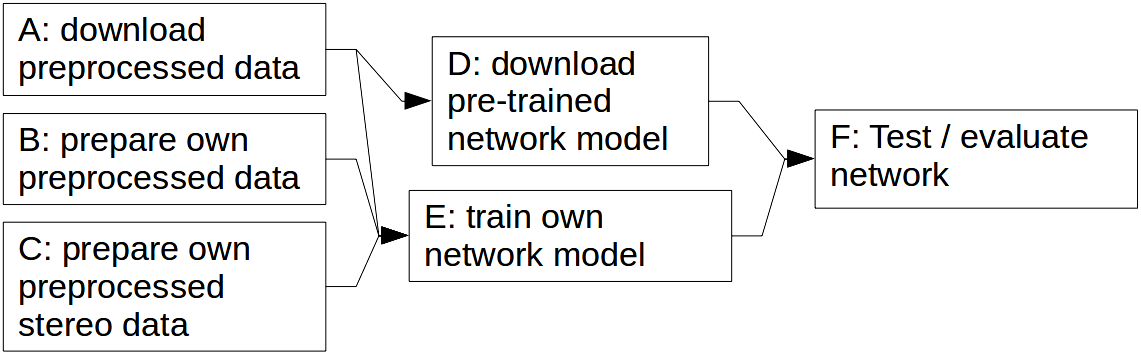
\includegraphics[width=1\textwidth]{../media/fpnet_paths_img.png}
    \caption{Various paths that were planned to simply transition from lidar-based 3D estimation to stereo-based 3D estimation. Generally, paths went chronologically as follow: ADF, AEF, BEF, and finally CEF.}
    \label{fp_paths}
\end{figure}

The most basic path, ADF, is simply using the given model to evaluate and achieve similar results to the official paper. Next, AEF used lidar pointclouds, but the model was trained locally. BEF required locally running the ``preprocessing" step, but was still functionally similar to the previous two paths. Finally, CEF truly deviates from the other paths by using a stereo-generated point cloud to preprocess data, then train on that, and finally evaluate the model's detection capability.

% NEWSECTION ===================================================================
\newpage
\section{Experiments}
\label{sect_experiments}
Once the network was built and implemented, several experiments were conducted and iterated upon in order to achieve the best possible performance with the given datasets and knowledge. The first subsection is dedicated to explaining the performance metrics of 3D object detection, then moves on to describing the results of each experiment and investigation performed with the network. As noted below and in the results of each experiment, the class ``Car" is the sole class that is examined. Other classes, such as Cyclist and Pedestrian, have evaluation code and even good ground truth labeling for them, but not in the sheer volume that the Car class has. Additionally, cars have the inherent benefit of having a generally uniform shape (box-shape body, wheels, etc). See Appendix \ref{appendix_kitti} for more information. All code used in both producing the results as well as the graphics of this paper are provided by \cite{gonzalez_smart3d_2019}. 

\subsection{Performance Metrics}
In order to determine the quality of results obtained, a few different metrics are implemented as are standard in practice. Here, the various metrics are explained, and in Appendix \ref{appendix_metrics} examples are provided. The concept of verifying accuracy in a statistical estimate is covered in \cite{manning_introduction_2008}, and some of this information is covered briefly below. In the field of image recognition, one particularly interesting metric is ``Intersection over Union", also referred to as IOU or Jaccard Index. From this metric, precision and recall may then be calculated. Precision and recall are fundamental in obtaining more abstracted metrics such as average precision (AP) and mean average precision (mAP), which are how different networks are compared. The following information is primarily taken from the well-known PASCAL VOC (visual objects classes) Challenge \cite{everingham_pascal_2010} and ``An Introduction to Information Retrieval" by \cite{manning_introduction_2008}.

\subsubsection{Defining an Outcome}
The first step in measuring performance is categorizing what a result may be. With a visual task such as object classification, there are 4 possible outcomes (all references to true/false positive/negatives in this document will be referred to as ``outcomes"), which will be  as shown below. In general, there may be a True Positive, False Positive, True Negative, or False Negative outcome. In practice, True Negatives are not used, and the remaining three are used to varying degrees. Each is better clarified as such:
\begin{itemize} \itemsep=-.5em
	\item True Positive: Correctly detecting a true object
	\item False Positive: Incorrectly detecting something that isn't there
	\item False Negative: Incorrectly ignoring a true object
	\item True Negative: Correctly ignoring something that isn't there
\end{itemize}

\begin{figure}[H]
	\centering
	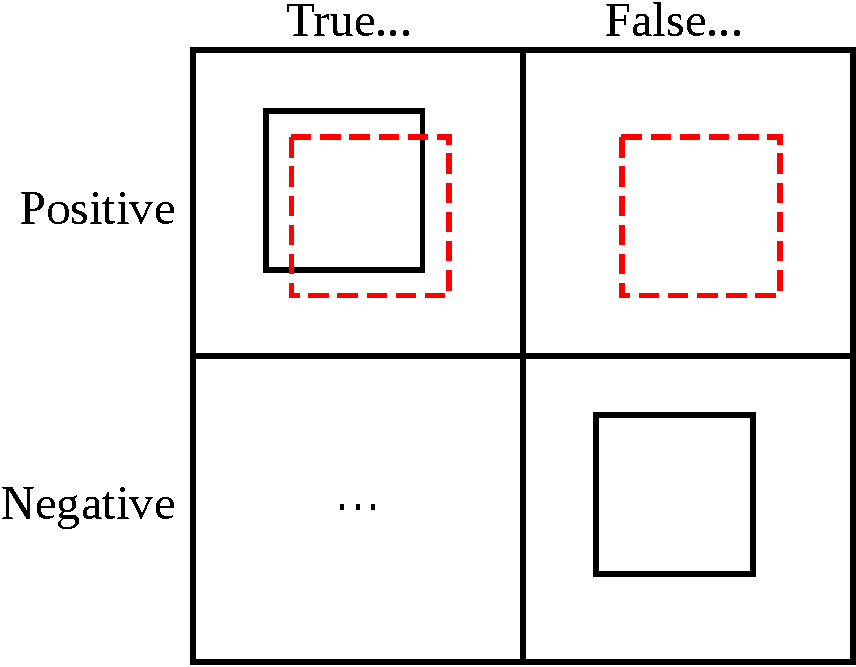
\includegraphics[width=.3\textwidth]{../media/tp_help.pdf}
	\caption{A visual representation of various outcomes, ground truths as solid black boxes and detections as dotted red boxes.}
	\label{tp_help}
\end{figure}

To actually classify a result in one of these categories, computer vision depends on using the overlap of a given bounding box estimate with a bounding box ground truth. If the overlap is above some threshold, the estimate is said to be a true positive. In some metrics, two estimates overlapping the same ground truth will only count the larger overlap, or the more confident estimate. This overlap is formally known as an Intersection over Union (IOU) value, or a Jaccard index.

\subsubsection{Intersection Over Union}
In image recognition, as well as other spatially-based tasks, accuracy is needed in various forms to know ``how well" a prediction overlaps, or matches, the ground truth. If, for example, an object-detection algorithm predicts the location of a car in a photo, one would like to know if such an estimate has any value, ideally with as few parameters as possible.

In light of this, IOU encompasses all relevant aspects of rating the overlap of two geometric shapes (e.g. rectangles) while enabling an intuitive, non-binary scoring of an estimate. IOU is calculated as two bounding regions' intersection over their union, just as the name states. Visually, this looks something like the below in Figure \ref{iou_img}. Uniquely, the calculation of area and intersection specifically for image boundaries is inclusive of the bounds, meaning that the length of a given difference must have ``+1" added to it.

In order to formally calculate IOU, a generalized form may be generated to apply to n-dimensions. The generalized mathematical equation is simply as follows. Given a region A and a region B:
\begin{equation}
IOU = \frac{|A\cap B|}{|A\cup B|} = \frac{|A\cap B|}{|A|+|B|- |A\cap B|}
\end{equation}

\begin{figure}[ht]
    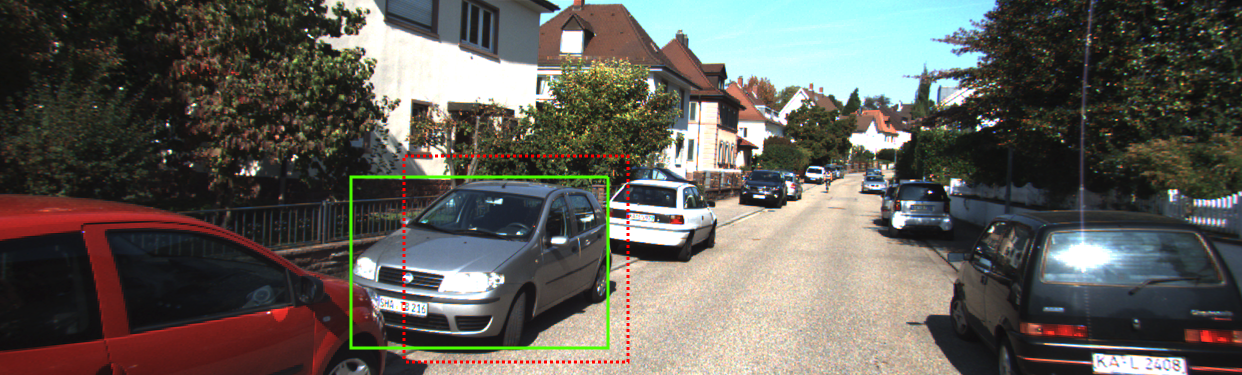
\includegraphics[width=1\textwidth]{../media/iou_img.png}
    \caption{Example of ground truth bounding box (solid green) and prediction bounding box (dashed red). In this image, the overlap between the green and red regions is the intersection, while the combined area is the union. The IOU of the two boxes is 0.64. Index 8 of the KITTI Object Detection dataset.}
    \label{iou_img}
\end{figure}

\subsubsection{Precision \& Recall}
\label{subsect_precrec}
Once all detections have been tallied and placed into their correct categories, their precision and recall may be calculated. In information retrieval, precision is defined as ``the fraction of retrieved documents that are relevant", and recall is defined as ``the fraction of relevant documents that are retrieved". Reworded for object detection: precision is the number of correct predictions divided by the total number of predictions, and recall is the number of correct predictions divided by the total number of possible answers. These two are also given as equations in terms of true positives and so on.

\begin{equation}
Precision = \frac{TruePositives}{TruePositives + FalsePositives}
\label{eq_prec}
\end{equation}

\begin{equation}
Recall = \frac{TruePositives}{TruePositives + FalseNegatives}
\label{eq_rec}
\end{equation}

Theoretically, precision and recall are generated at multiple points by varying a probability threshold and graphing each result. In practice, a precision-recall curve is generated by a more complex process that involves taking the cumulative sum of the detections in order of descending confidence level (1.0,0.99, ...). Once a precision vector and a recall vector have been created, the plot may appear something like below, reproduced from Figure \ref{precrec_steps} in Appendix \ref{appendix_metrics}. 

\begin{figure}[H]
	\centering
	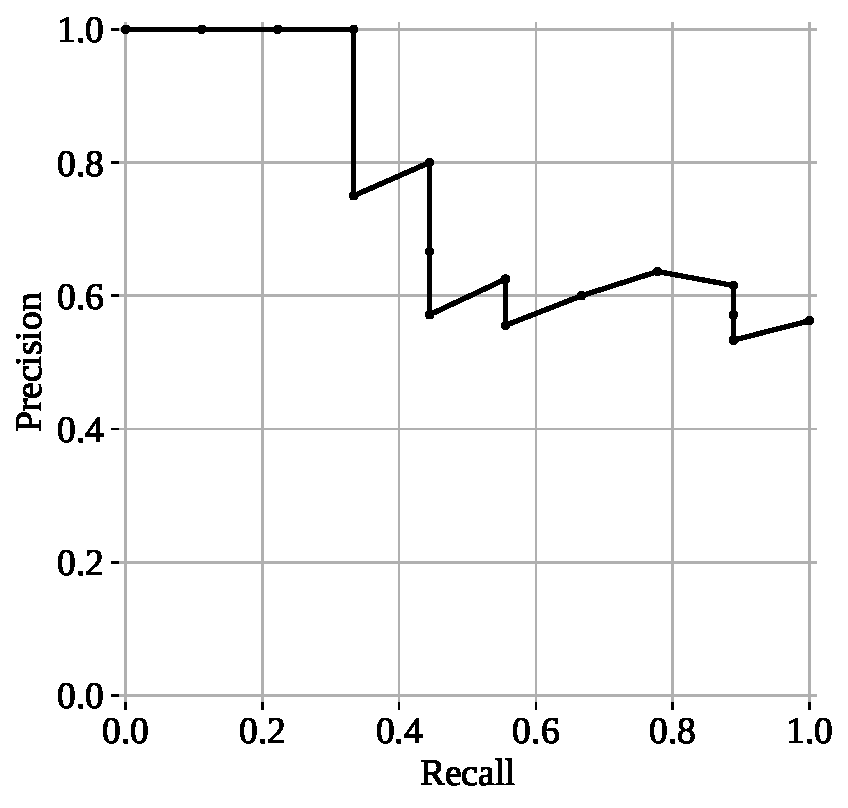
\includegraphics[width=0.4\linewidth]{../media/precrec_steps.pdf}
	\caption{A typical precision-recall curve. Taken from the example in Appendix \ref{appendix_metrics}.}
\end{figure}


\subsubsection{Calculating Average Precision}
Once a set of recall and precision data has been calculated, then AP is a fast and simple calculation. Formally, average precision is defined as the area beneath a precision-recall curve. However, this metric has been calculated in various forms and often modified by the scientific community, including the previously common 11-point average precision used by the Visual Objects Challenge (VOC), used until 2009 and by several subsequent object recognition challenges. 11-point AP has been argued to be slightly more robust against very jittery curves, but also judges results rather ``crudely" and less accurately \cite{everingham_pascal_2015}. For the purposes of computer vision, AP may also be considered a weighted sum of precision, considering that the differences in recall value may be used as the weights since their sum is 1. Thus, to match the function output by \cite{pedregosa_scikit-learn:_2011}, one may simply take a rectangular numerical integration of the values in Table \ref{precrec_ans}. It must be kept in mind that the order of the values MUST be in order of ascending recall value. The mathematical formula for calculating AP is then given in \ref{eq_ap}, where 1 is the starting index and $n$ is the length of the vector:

\begin{equation}
AP = \sum^{n-1}_{i=1} ({re}_{i+1}-{re}_{i})({pr}_{i+1})
\label{eq_ap}
\end{equation}

\subsection{Experiment 1: Lidar-Based Performance as a Baseline}

To first properly understand the performance capability of lidar-based 3D object detection, the typical pipeline was first verified locally. There are multiple setup steps as given by the authors, with a specific training-validation split. This was followed, and the performance was indeed on par with what exists officially on the KITTI 3D Object Detection benchmark. As described in Figure \ref{fp_paths}, there are three paths that emulate the methodology official results, all of which use lidar as the source of point cloud information: 

\begin{itemize} \itemsep=-0.5em
	\item ADF (downloading the pretrained model and evaluating immediately)
	\item AEF (download preprocessed data, train network, and evaluate)
	\item BEF (prepare preprocessed data, train network, and evaluate)
\end{itemize}

Aside from path ADF, which of course features no training component, the training loss of each path is visualized below in Figure \ref{fpnet_loss1}. path ``AEF" was performed twice (revision 0 and revision 1), during different times in the project; The performance remained relatively consistent, however.

\begin{figure}[H]
	\centering
	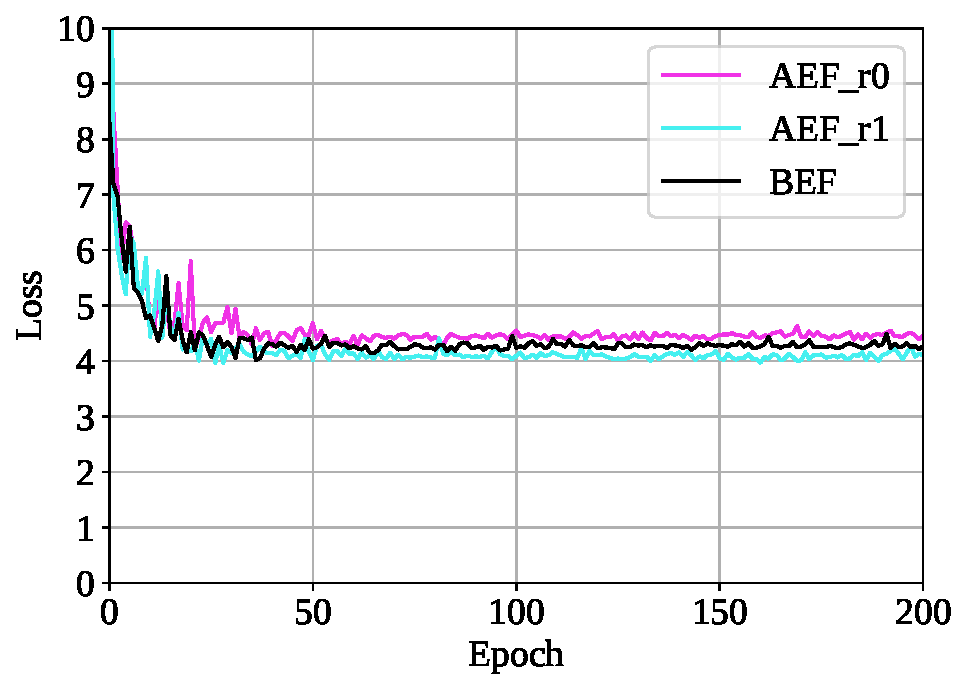
\includegraphics[width=0.6\linewidth]{../media/fpnet_loss1.pdf}
	\caption{Loss over epochs graph for Experiment 1. Run AEF\_r1 achieved the lowest training loss, settling to a value of around 4.1. The loss value represents an average score of how much a network predicts incorrectly during training.}
	\label{fpnet_loss1}
\end{figure}

Taking a slightly closer look at the training data, the lowest value loss that the network achieved while training was 4,1. The rate at which loss was changing also seemed to decrease to zero, indicating that the network was quite stable in its weights by the end of the training. For future reference, path BEF will be used to compare to other networks since it performed the best of these run paths.

Additionally, the precision-recall curve of each path for the ``Car" class is also shown in Figure \ref{fpnet_pr1}. The curves generally indicate that the lidar-based point clouds were quite robust, and the AP score for the three paths are as follow.

\begin{table}[ht]
	\centering
	\caption{FPNet lidar-based results, across varying difficulties. BEF performed marginally better than the other runs, and was thus used as a reference in future experiments. AP score is calculated by finding the area under the precision-recall curve.}
	\begin{tabular}{|c|c|c|c|}
		\hline
		\b{Path} & \b{AP\_Easy} & \b{AP\_Med} & \b{AP\_Hard} \\ \hline
		  ADF    &    84.07     &    71.28    &    63.35     \\ \hline
		  AEF0   &    82.59     &    68.72    &    61.25     \\ \hline
		  AEF1   &    83.51     &    68.99    &    61.04     \\ \hline
		  BEF    &    84.12     &    71.00    &    63.27     \\ \hline
	\end{tabular}
	\label{fpnet_ap1}
\end{table}


\begin{figure}[H]
	\centering
	\subfigure[]{
	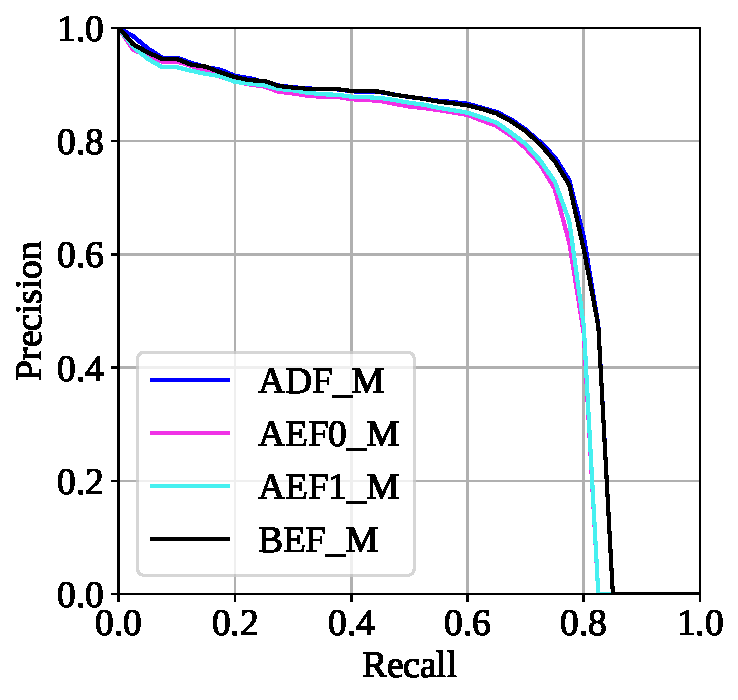
\includegraphics[width=0.4\linewidth]{../media/fpnet_pr1_multi.pdf}}
	\subfigure[]{
	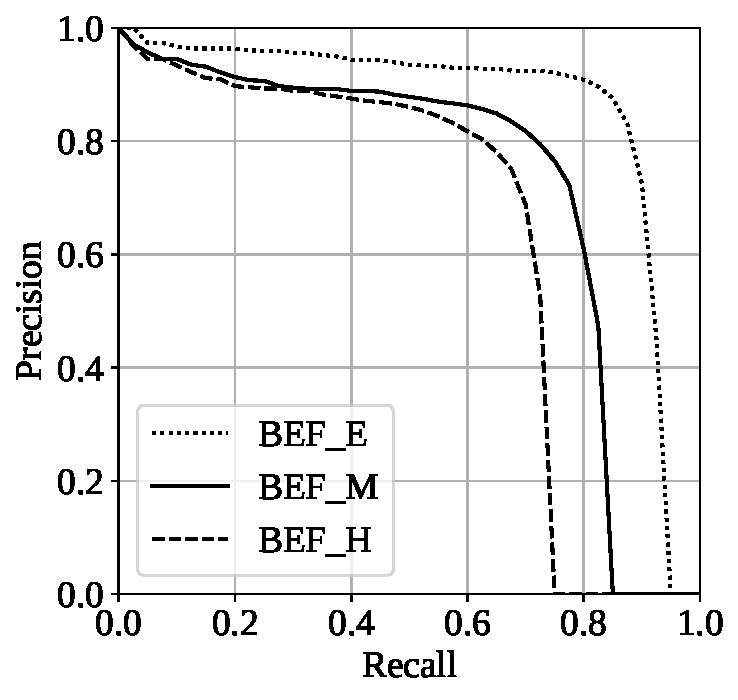
\includegraphics[width=0.4\linewidth]{../media/fpnet_pr1_bef.pdf}}
	\caption{Precision recall curves for Experiment 1. Subfigure (a) shows various runs at compared medium difficulty, while Subfigure (b) shows the best-performing run BEF at Easy, Moderate, and Hard difficulties.}
	\label{fpnet_pr1}
\end{figure}

Given that these are results from a lidar-based network, they are therefore the benchmark against which performance was then measured. 

\subsection{Experiment 2: Stereo-Based Performance, using Stereo Dataset}
The first experiment had the objective of using the stereo network, once trained, to provide a new source of point cloud data. This experiment corresponds with the path ``CEF": preparing preprocessed data with stereo vision instead of lidar, train the network model on this information, then evaluate the network performance. Because this experiment was later further modified, it is known as CEF\_r0, while the second version is named CEF\_r1. 


The training loss is provided below in Figure \ref{fpnet_loss2}, with a comparison to previous the previous, lidar-based path ``BEF". 

\begin{figure}[ht]
	\centering
	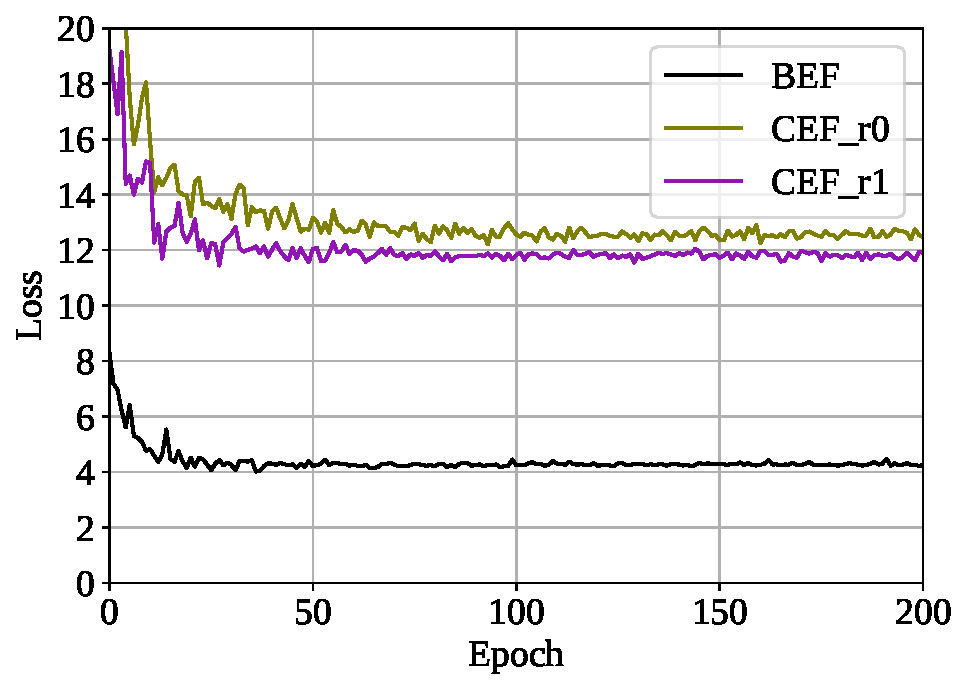
\includegraphics[width=0.6\linewidth]{../media/fpnet_loss2.pdf}
	\caption{Loss over epochs graph for Experiment 2. Run CEF\_r1 achieved the lowest final loss value, although reference curve BEF shows that lidar-based methods typically achieve lower loss during training.}
	\label{fpnet_loss2}
\end{figure}

As can be seen from the figure, the training loss also reached a point of equilibrium and ceased decreasing after some time, but at a much higher value than path BEF. CEF\_r0's loss value instead settled closer to a value of 12.4. 

In the evaluation, CEF\_r0 performed at a significantly lower level than BEF, indicating a need to further refine the model. However, there is some promise in this result, as it indicates that the system does perform well in the ``Easy" mode, when cars are generally within 30 meters of the sensor. The results from this experiment, as well as further reading, motivated the next experiment conducted. This is shown below, in Figure \ref{fpnet_pr2}.

After the initial results CEF\_r0, the 3D reconstruction step was reexamined for any possible errors. It was then discovered that PSMnet internally crops stereo image pairs into a standardized size, a significant piece of previously unmentioned information. The primary cause of non-standardized image sizes in the object detection dataset is due to the rectification performed on each raw image. This means that the images, after being rectified, are then cropped in a non-standardized way to remove the resulting non-image regions. PSMnet itself only works on a standardized image size, so it therefore takes the smallest dimensions across the dataset and crops all image pairs to that size, [1232,368] pixels. The PSMnet crop is anchored at the bottom-right corner of each image, which provides some consistency but may still contribute to a source of error, since the exact method of cropping both rectified data and images for stereo processing are not totally aligned. A second and lesser source of possible error that was corrected in CEF\_r1 was the method of reconstruction used. This updated method is reflected in \ref{sect_reconstruct}. The constant being used for all disparity-to-depth transformations was consistent, rather than being the product of baseline and $F_U$, horizontal focus length. Thus, Figure \ref{fpnet_pr2} and Table \ref{fpnet_ap2} show the improvement from CEF\_r0 to CEF\_r1. 

\begin{table}[ht]
	\centering
	\caption{Experiment 2 results, with Frustum Pointnets using stereo data. Average precision shown for the first two attempts, across varying difficulties, for the Car class.}
	\begin{tabular}{|c|c|c|c|}
		\hline
		\b{Path} & \b{AP\_Easy} & \b{AP\_Med} & \b{AP\_Hard} \\ \hline
		CEF0   &    35.61     &    23.02    &    20.43     \\ \hline
		CEF1   &    42.57     &    28.60    &    24.07     \\ \hline
	\end{tabular}
	\label{fpnet_ap2}
\end{table}

\begin{figure}[H]
	\centering
	\subfigure[]{
		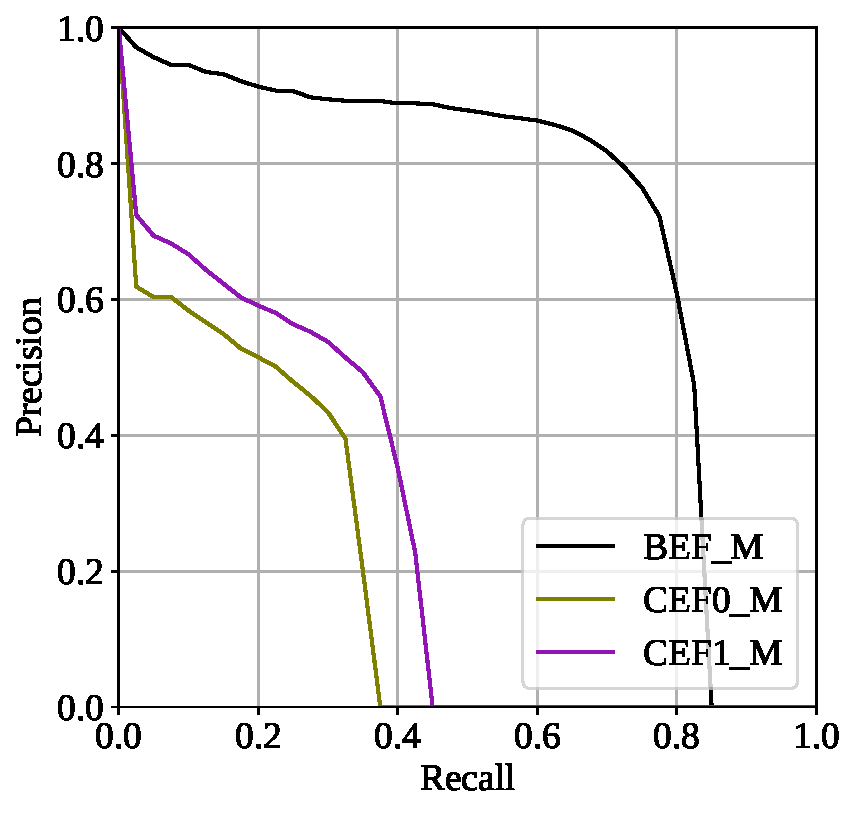
\includegraphics[width=0.4\linewidth]{../media/fpnet_pr2_multi.pdf}}
	\subfigure[]{
		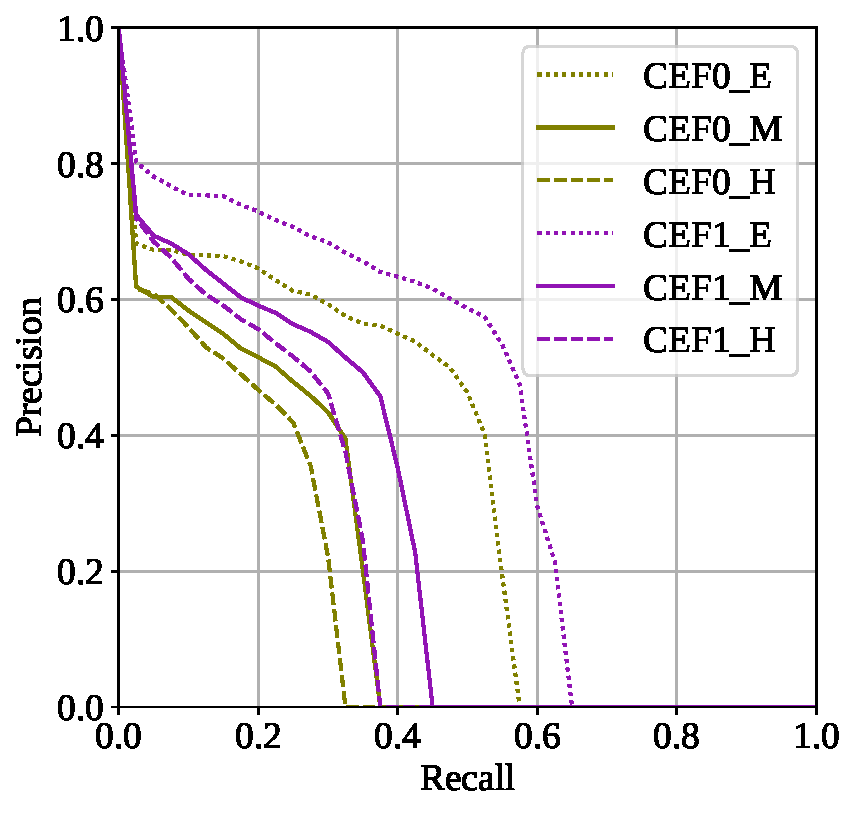
\includegraphics[width=0.4\linewidth]{../media/fpnet_pr2_cef01.pdf}}
	\caption{Precision-recall graphs for both CEF\_r0 and CEF\_r1, with lidar-based result BEF also shown for reference. In (a), the improvement between r0 and r1 manifests in an $AP_M$ increase of 5 percentage points, and at ``Easy" difficulty, the best curve in (b) has an AP of 42.57.}
	\label{fpnet_pr2}
\end{figure}

\subsection{Experiment 3: Stereo-Based Performance, using Object Detection Dataset}
Upon reviewing the most closely related paper, by \cite{wang_pseudo-lidar_2019}, the suggestion of changing the training dataset for PSMnet was taken. A pretrained stereo model was once again taken, directly from the authors, and finetuned exclusively on the same training split used by FPnet. This is in contrast to the original KITTI stereo dataset, used by the authors. The reasons for this are given below as well as further clarified in Appendix \ref{appendix_kitti}.

\subsubsection{Similarity of Ground Truths Across Datasets}
\label{sect_datamod}
After the initial evaluation, the network was prepared and trained on KITTI data. The original authors of PSMnet provide a model pre-trained on the Freiburg SceneFlow dataset; this model was also used. After this step, however, it must be clarified that there are images in the KITTI stereo dataset that overlap greatly in similarity to those in the KITTI object detection dataset. The difference between the two datasets are essentially that one has been optimized for object detection, and the other for stereo disparity map estimation. This similarity was also noted in \cite{wang_pseudo-lidar_2019}, and this paper took the same approach to make corrections, as described below. Figure \ref{similarity_stereo_objdet} below also demonstrates the similarity between two sample images, which points to the risk of having a part of the network trained on what may be validation or even evaluation data. This would result in data leakage and thus put the validity of the results into question.

\begin{figure}[ht]
	\centering
	\subfigure[000132\_10 from Stereo]{
		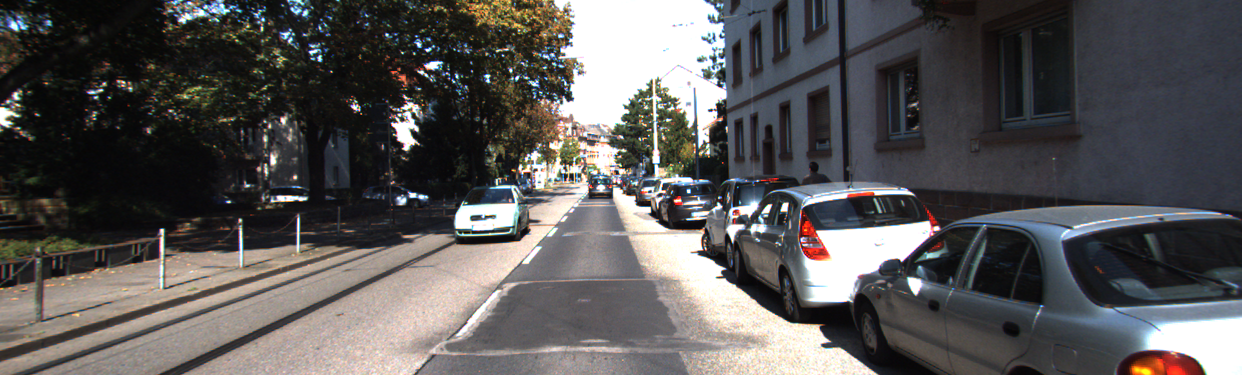
\includegraphics[width=1\linewidth]{../media/similar_000132_10_stereo.png}}
	\subfigure[000286 from ObjDet]{
		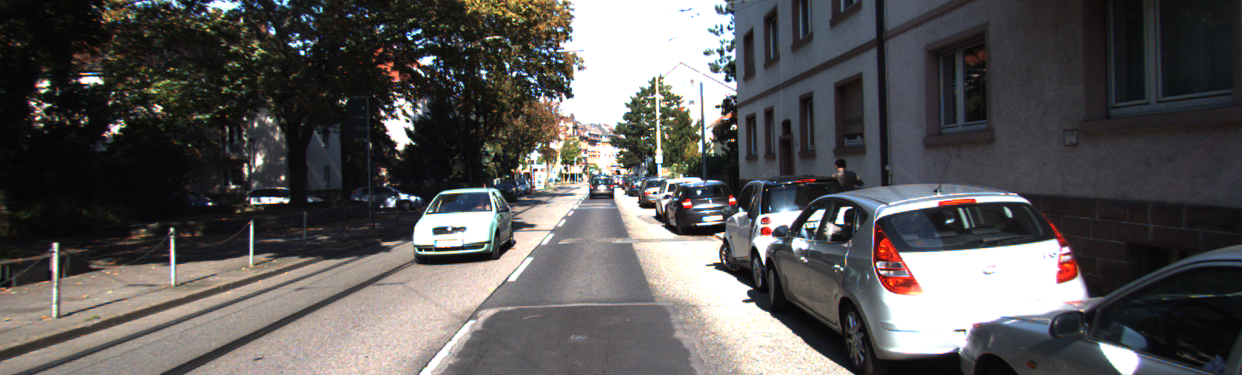
\includegraphics[width=1\linewidth]{../media/similar_000286_objdet.png}}
	\caption{Example of how two unique records from the separate datasets have overly-similar scenes. There are multiple examples of this, which creates the motivation to generate a secondary set of disparity ground truths for the object detection dataset}
	\label{similarity_stereo_objdet}
\end{figure}

In order to deal with the dataset overlap, the KITTI object detection dataset was adapted to be used for training stereo data. Lidar data was projected onto the left image plane, cropped to the original image bounds, converted to integer values, then multiplied by a constant. These steps are in line with both the way that \cite{wang_pseudo-lidar_2019} were able to generate their self-made stereo ground truths as well as how the KITTI dataset authors generated their ground truth, as described in the stereo development kit. Locations in the image that have no lidar data are left alone at a value of 0.0, and finally the resulting array is saved to a PNG image file format containing integer values. Please refer to the generation script in the repository for the exact steps used to generate the pseudo ground truth stereo images \cite{gonzalez_smart3d_2019}.

\subsubsection{Results of Modification}
It was discovered at some point that the training / validation data used in the KITTI stereo image set was overlapping too much with images used in the KITTI object detection task. Thus, \cite{wang_pseudo-lidar_2019} was referred to and guided the change in retraining PSMnet. The difference in training is shown below.

Figure \ref{psmnet_star_train_info} below shows the loss throughout the training of PSMnet on the object detection dataset, also known as PSMstar (based on the similar name given by Wang et al \cite{wang_pseudo-lidar_2019}, as well as the original stereo dataset model for reference. 

\begin{figure}[ht]
	\centering
	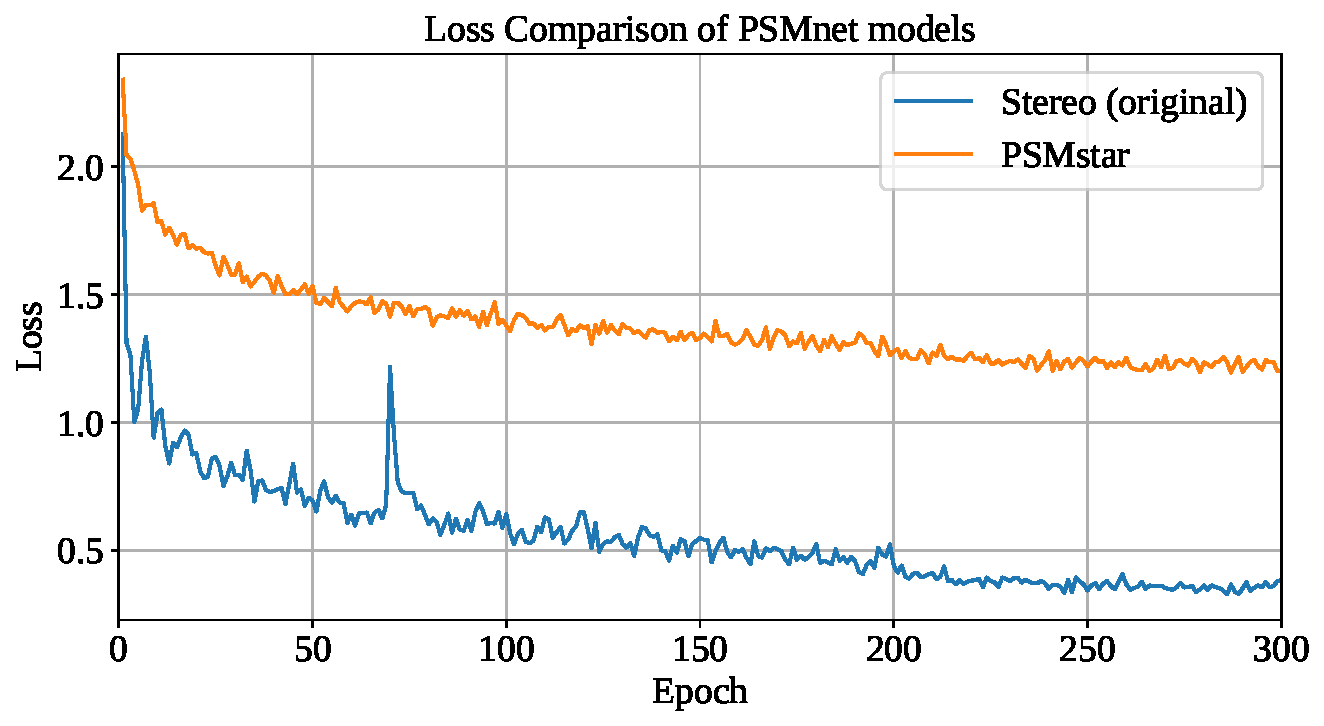
\includegraphics[width=0.7\linewidth]{../media/info_psmnet_comparison_Loss.pdf}
	\caption{Loss graphs for both the original stereo-dataset PSMnet model and the retrained, object-detection-based ``PSMstar" model. The average difference between the two curves is a loss of about 0.82. The higher loss for PSMstar may result from using self-made ground truth labels rather than using the more detailed stereo dataset versions.}
	\label{psmnet_star_train_info}
\end{figure}

In addition to the quantitative difference in training, a qualitative difference in the estimation pattern may be seen below, in Figure \ref{new_psmnet}. Overall, the change in quality may be seen as a more detailed but less contrasting depth map.

\begin{figure}[H]
	\centering
	\subfigure[Stereo estimation with original PSMnet model]{
		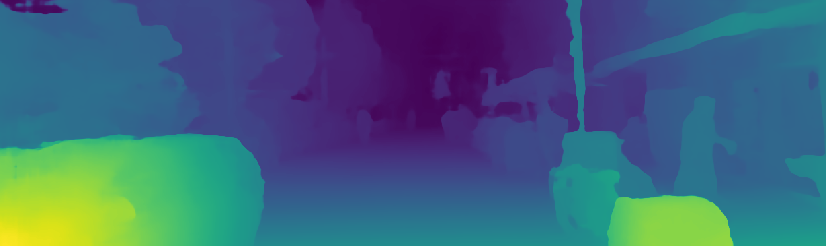
\includegraphics[width=1\linewidth]{../media/ind15_psmnet_v190308_AsOf190626.png}}
	\subfigure[Stereo estimation with new PSMnet model]{
		
\includegraphics[width=1\linewidth]{../media/ind15_psmstar_v190613_AsOf190626.png}}
	\caption{Comparison of old and new model for PSMnet. Index 15 of the KITTI Object Detection dataset. There are typically less extreme values, yet also some higher contrast in the low (distant) values, as visible by a more clear outline of two pedestrians in the center of the image. See Figure \ref{reconstruction}(a) for photo reference.}
	\label{new_psmnet}
\end{figure}

The training loss of the modified FPnet is provided below in Figure \ref{fpnet_loss3}, once again with run BEF plotted for reference. Runs CEF\_r2 and CEF\_r3 are nearly identical, although a slight modification was tested out with CEF\_r3: removing all points in the stereo-generated point cloud that were 1 meter above the sensor vertical height. However, the decrease of information, whatever its quality, seems to have had a very slight negative impact rather than positive one on the overall result.

\begin{figure}[ht]
	\centering
	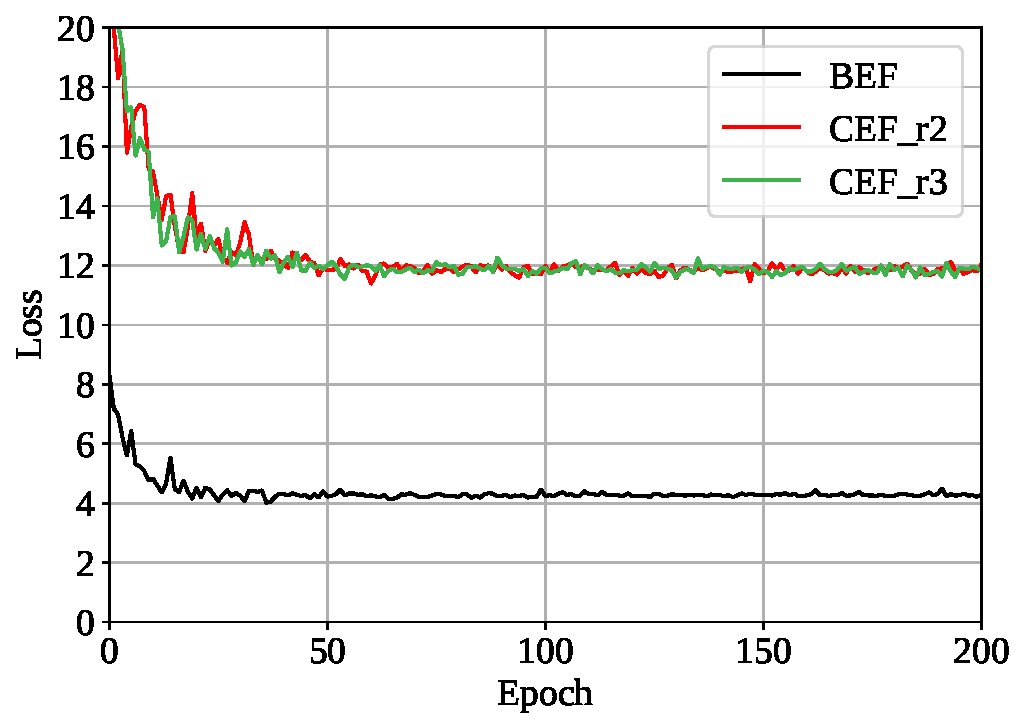
\includegraphics[width=0.6\linewidth]{../media/fpnet_loss3.pdf}
	\caption{Loss over epochs graph for Experiment 3. Run CEF\_r2 and r3 both ended training with a final loss of about 12.0. However, this value is still much higher than the reference BEF training loss.}
	\label{fpnet_loss3}
\end{figure}


The precision-recall curves for the ``Car" class is given below in Figure \ref{fpnet_pr3}, including one only for CEF\_r3, as well as the AP scores for the various difficulties in Table \ref{fpnet_ap3}.

\begin{table}[ht]
	\centering
	\caption{Experiment 3 results, with FPNet stereo-based results. Runs r2 and r3 shown across varying difficulties.}
	\begin{tabular}{|c|c|c|c|}
		\hline
		\b{Path} & \b{AP\_Easy} & \b{AP\_Med} & \b{AP\_Hard} \\ \hline
		CEF2   &    47.41     &    30.69    &    25.15       \\ \hline
		CEF3   &    45.43     &    30.45    &    24.29       \\ \hline
	\end{tabular}
	\label{fpnet_ap3}
\end{table}

\begin{figure}[H]
	\centering
	\subfigure[]{
		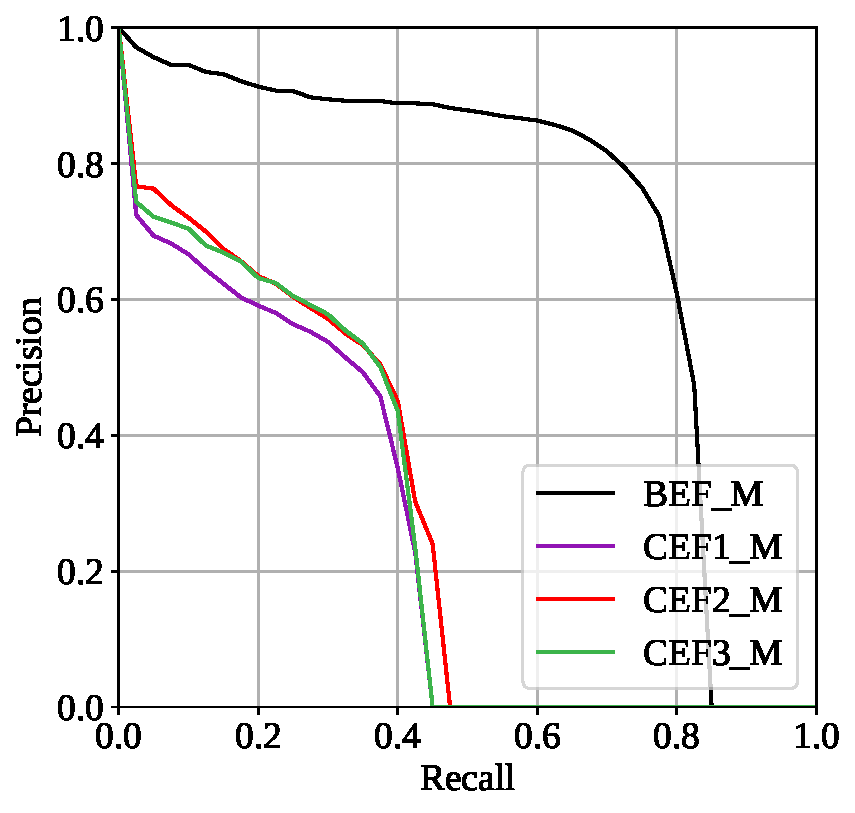
\includegraphics[width=0.4\linewidth]{../media/fpnet_pr3_multi.pdf}}
	\subfigure[]{
		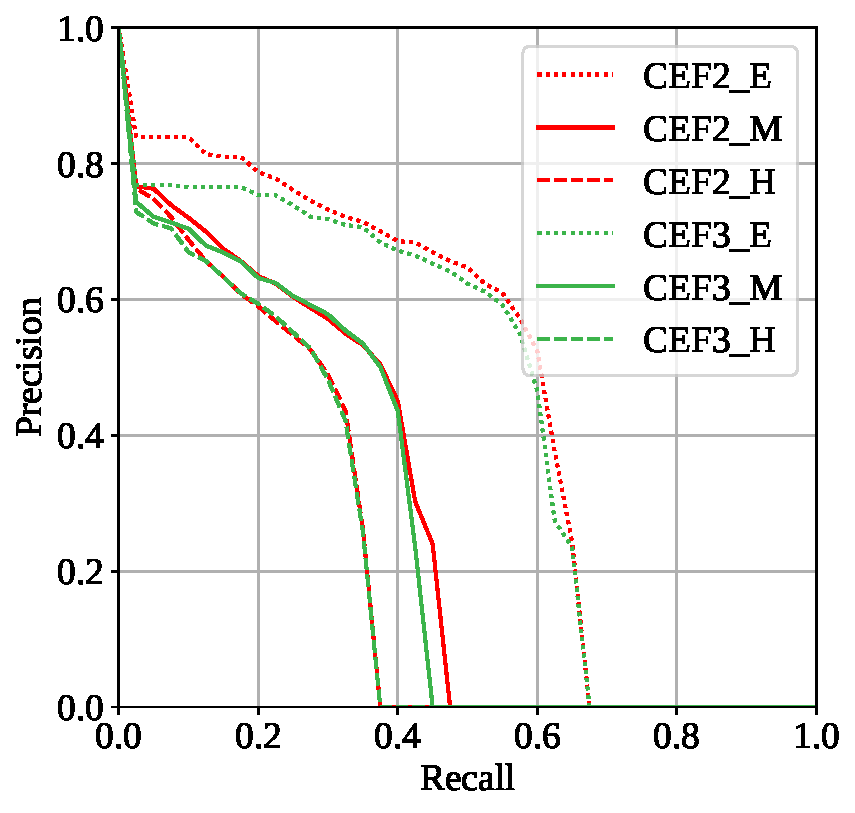
\includegraphics[width=0.4\linewidth]{../media/fpnet_pr3_cef23.pdf}}
	\caption{Precision-recall graphs for both CEF\_r2 and CEF\_r3 in (a), with lidar-based result BEF also shown for reference. Subfigure (b) further shows both across the Easy, Moderate, and Hard difficulties.}
	\label{fpnet_pr3}
\end{figure}

Although the results still lag behind lidar-based performance, Table \ref{fpnet_ap3} shows yet another improvement in AP from CEF\_r1 to CEF\_r2, improving by about 5 percentage points on ``Easy", 2 points on ``Medium", and 1 point on ``Hard".


\subsection{Comparison with Other Networks} 
In addition to both developing and testing ``SPCLnet", the official performance data of other networks was downloaded, graphed, and compared. In addition to the self-made network, the following networks were compared: 
\begin{itemize}
	\item Pseudo-Point Cloud network, by \cite{wang_pseudo-lidar_2019}
	\item STD: Sparse-to-Dense 3D Object Detector for Point Cloud, \cite{yang2019std}
	\item RCNN Stereo Network, by \cite{li_stereo_2019}
	\item RT3D: Real-time 3D vehicle detection, by \cite{zeng2018rt3d}
\end{itemize}

\begin{table}[ht]
	\centering
	\caption{Results achieved by other notable networks on the KITTI dataset.}
	\begin{tabular}{|c|c|c|c|}
		\hline
		\b{Path} & \b{AP\_Easy} & \b{AP\_Med} & \b{AP\_Hard} \\ \hline
		  STD    &    86.61     &    77.63    &    76.06     \\ \hline
		  WANG   &    55.40     &    37.17    &    31.37     \\ \hline
		  RCNN   &    49.23     &    34.05    &    28.39     \\ \hline
		  RT3D   &    28.50     &    24.10    &    20.32     \\ \hline
	\end{tabular}
	\label{fpnet_ap4}
\end{table}

\begin{figure}[H]
	\centering
	\subfigure[]{
		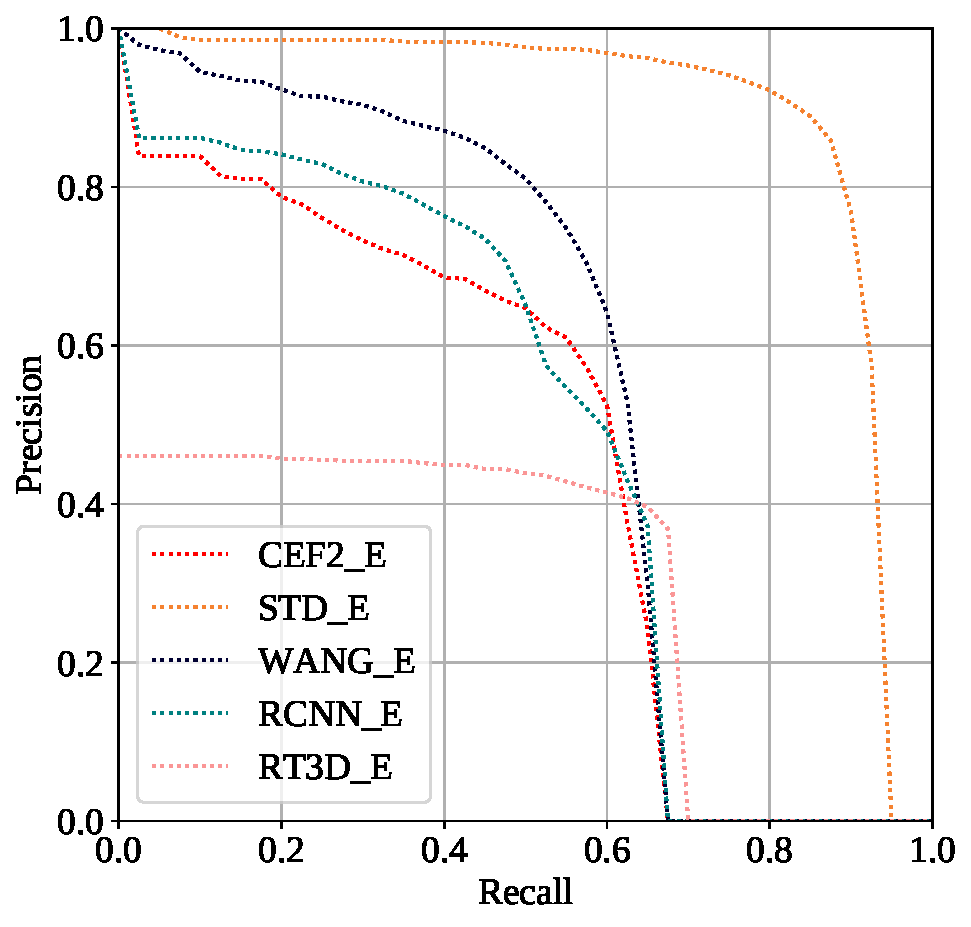
\includegraphics[width=0.487\linewidth]{../media/fpnet_pr4_multi_e.pdf}}
	\subfigure[]{
		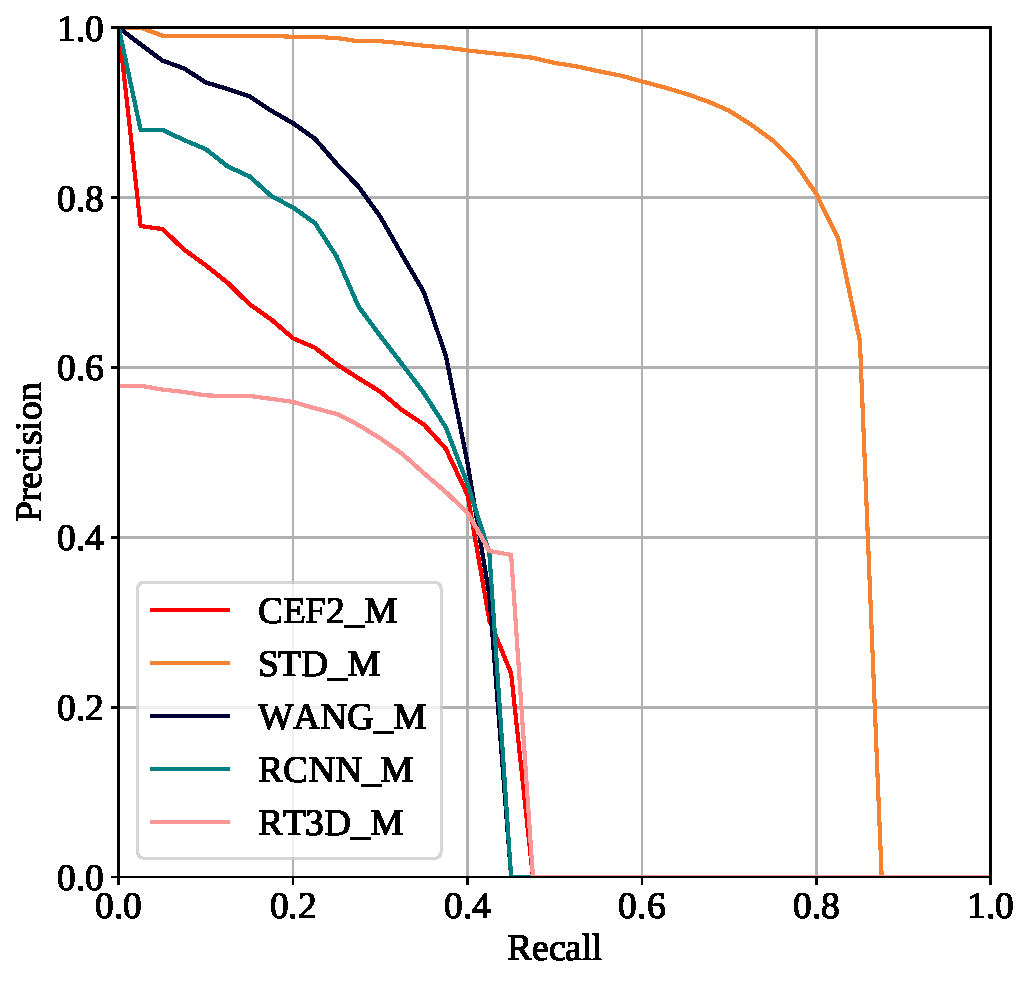
\includegraphics[width=0.487\linewidth]{../media/fpnet_pr4_multi_m.pdf}}
	\caption{Precision-recall graphs. Subfigure (a) compares run CEF\_r2 to other notable networks at Easy  difficulty. Subfigure (b) compares the same set at Moderate difficulty.}
	\label{fpnet_pr4}
\end{figure}

The best performing iteration of SPCLnet, CEF\_r2, while not performing the outright best, shares some interesting characteristics with the other stereo networks. For one, there is a sharp decline at the top-left of the curve, a trait that the RCNN curve also shares. This is typically caused when the threshold to determine outcomes is higher, occurring at higher precision and lower recall values. In addition to this, all stereo algorithms reach 0.0 precision at approximately the same recall value, at each given difficulty (0.5 recall at Moderate, 0.7 at Easy). This would indicate that even when the threshold is nearly nonexistent, there simply aren't enough valid detections to outweigh the number of False Negatives. 

% NEWSECTION ===================================================================
\newpage
\section{Conclusions and Future Work}
\label{sect_conclusions}
%1. stereo vision can compete with lidar, in near-range applications
%2. KITTI dataset not enough today
%3. the quality of a disparity map is key
%4. real-time stereo is approaching, but not without simplification and optimization

The main effort of this thesis has gone towards asking one general question: can stereo vision reasonably provide an alternative to lidar sensors in the realm of 3D detection? There are two specific conclusions that have been drawn from the literature as well as this work, specifically: Stereo vision can potentially compete with lidar as a viable distance sensor at relatively short distances, and the quality of the disparity data has a strong impact on the final results (and is a source of possible future work). Additional future work lies in real-time applications, which are within reach. 

Stereo vision cameras may always trail a lidar sensors in terms of quality, but there is a cost-quality tradeoff that becomes appealing under certain circumstances. As can be seen by the results in Table \ref{fpnet_ap3} and Table \ref{fpnet_ap4}, stereo-based networks suffer a larger decrease in performance when compared between the ``Easy" and ``Moderate" difficulties (corresponding to objects located within 30 meters and objects located beyond 30 meters, respectively). Figure \ref{corr_pct_within} also demonstrates that as lidar reference distance increases, the fraction of stereo points correctly within error bounds decreases. There are large strides being made in the field, from pure stereo approaches \cite{zeng2018rt3d,li_stereo_2019} to macro-networks that draw inspiration from lidar based approaches \cite{wang_pseudo-lidar_2019}. Throughout the duration of this paper's writing, there have already been a few new submissions to the KITTI dataset, indicating a growing interest in this subfield. 



There are several sources and explanations for the disparity in accuracy, the most prominent being the quality of the disparity map estimator itself. This paper and Wang et al. \cite{wang_pseudo-lidar_2019} both utilized PSMnet, but the likelihood of small differences in configuration between the two may have resulted in significant performance differences. The second major source of stereo camera error may lie in the KITTI dataset source images. Minor inaccuracies at even a few pixels can degrade system performance, and thus more investigation is needed into generating the most accurate disparity map and subsequent point cloud possible. Clearly, the latter half of SPCLnet and the pseudo-point cloud network by \cite{wang_pseudo-lidar_2019}, Frustum Pointnets by \cite{qi_frustum_2017}, can achieve near state-of-the-art results when given the right information, i.e. accurate point cloud. Looking at Figure \ref{fpnet_pr4}, all stereo networks seem to have an upper limit on performance: none perform beyond a certain recall level, such as 0.5 at Moderate difficulty. This presents an opportunity to explore new datasets that include both lidar and stereo image data. As of now, the KITTI object detection dataset, initially published in 2012 \cite{geiger_are_2012}, is roughly 7 years old, and most of the images on this dataset are about 0.5 megapixels (MP) in resolution. This is simply not enough to provide adequate information for generating a disparity map, aside from apparent need to generate one's own set of ground truth data from the object detection dataset in order to even train a stereo network on it. New datasets are showing some level of promise, such as the Apolloscape dataset \cite{huang_apolloscape_2018} or even moderately aged datasets such as \cite{cordts_cityscapes_2016}, and future research would benefit greatly from the inclusion of disparity map ground truth data.

Real-time stereo-based 3D estimation is within reach for a few simple reasons. For one, there are already real-time stereo disparity map estimators and commercial products, although their ouput is generally only a point cloud at best, if not a disparity map. Next, optimizations may be made in the network architecture presented in this paper. The data are transformed several times when moving between the 2.5D disparity map format to the 3D point cloud format, and this may be simplified in a unified pipeline, such as moving the reconstructon step to a later point with a subset of points. 


